%==============================================================
%  EE201 -- Circuit Theory I
%  Lecture 15 : Nonlinear Resistive Circuits -- slides
%  M. Mert Ankaralı, METU EEE
%
%  Compile:  ./build.sh      (or: pdflatex EE201_Lecture_15_slides.tex, twice)
%  Same colour code as the handout:
%      charge = purple, current = blue, voltage = orange, power = green
%==============================================================
\documentclass[11pt,aspectratio=169]{beamer}

\usepackage{appendixnumberbeamer}
\usepackage[T1]{fontenc}
\usepackage[utf8]{inputenc}
\usepackage[english]{babel}
\usepackage{lmodern}
\usepackage{amsmath,amssymb}
\usepackage{booktabs}
\usepackage{array}
\usepackage{colortbl}
\usepackage{tikz}
\usepackage[american,siunitx]{circuitikz}
\usetikzlibrary{matrix,arrows.meta,positioning,calc,decorations.pathreplacing,decorations.pathmorphing,decorations.markings}
\usetikzlibrary{overlay-beamer-styles}

%-------------------- plain METU-flavoured theme --------------
\usetheme{default}
\usecolortheme{default}
\useinnertheme{rectangles}
\setbeamertemplate{navigation symbols}{}
\setbeamertemplate{itemize items}[square]
\setbeamerfont{frametitle}{size=\large,series=\bfseries}
\setbeamerfont{title}{size=\LARGE,series=\bfseries}

\definecolor{metured}{RGB}{155,27,48}
\definecolor{metugray}{RGB}{88,89,91}
\definecolor{metulight}{RGB}{243,240,241}
\definecolor{ccur}{RGB}{0,102,170}
\definecolor{cvolt}{RGB}{214,120,0}
\definecolor{cpow}{RGB}{23,128,74}
\definecolor{ccharge}{RGB}{124,60,160}
\definecolor{cflux}{RGB}{0,138,138}
\definecolor{copper}{RGB}{184,98,30}

\setbeamercolor{structure}{fg=metured}
\setbeamercolor{frametitle}{fg=metured,bg=}
\setbeamercolor{title}{fg=metured}
\setbeamercolor{normal text}{fg=black!88}
\setbeamercolor{block title}{fg=white,bg=metured}
\setbeamercolor{block body}{bg=metulight}
\setbeamercolor{alerted text}{fg=metured}

\setbeamertemplate{frametitle}{%
  \vspace{0.55em}%
  \usebeamerfont{frametitle}\usebeamercolor[fg]{frametitle}\insertframetitle\par
  \vspace{-0.2em}{\color{metured}\rule{\textwidth}{1pt}}\par\vspace{-0.2em}}

\setbeamertemplate{footline}{%
  \hbox{\begin{beamercolorbox}[wd=\paperwidth,ht=2.4ex,dp=1.4ex,leftskip=1.2em,rightskip=1.2em]{}%
  \tiny\color{metugray}\coursecode\ \textbar\ Lecture 15: Nonlinear Resistive Circuits
  \hfill \insertframenumber/\inserttotalframenumber
  \end{beamercolorbox}}}

%-------------------- macros ----------------------------------
\newcommand{\coursecode}{EE201}
\newcommand{\term}{Fall 2026--2027}
\newcommand{\Icol}[1]{\textcolor{ccur}{#1}}
\newcommand{\Vcol}[1]{\textcolor{cvolt}{#1}}
\newcommand{\Pcol}[1]{\textcolor{cpow}{#1}}
\newcommand{\Qcol}[1]{\textcolor{ccharge}{#1}}
\newcommand{\Fcol}[1]{\textcolor{cflux}{#1}}
\newcommand{\uni}[1]{\,\mathrm{#1}}
\newcommand{\A}{\uni{A}} \newcommand{\V}{\uni{V}}
\newcommand{\W}{\uni{W}} \newcommand{\J}{\uni{J}}
\newcommand{\Cb}{\uni{C}} \newcommand{\s}{\uni{s}}
\newcommand{\Wb}{\uni{Wb}} \newcommand{\Hy}{\uni{H}}
\newcommand{\Sie}{\uni{S}}


%  voltage sources: smaller + and - inside the circle, further apart
\ctikzset{bipoles/vsourceam/inner plus={\tiny$+$},
          bipoles/vsourceam/inner minus={\tiny$\vphantom{+}-$},
          bipoles/vsourceam/margin=0.85,
          bipoles/cvsourceam/inner plus={\tiny$+$},
          bipoles/cvsourceam/inner minus={\tiny$\vphantom{+}-$},
          bipoles/cvsourceam/margin=0.85}
\ctikzset{bipoles/length=0.9cm, label/align=straight,
          bipoles/generic/height=0.28, bipoles/generic/width=0.62}
\tikzset{
  iar/.style={-{Stealth[length=2.2mm]}, ccur, thick},
  glab/.style={font=\footnotesize, text=metured},
  ttl/.style={font=\scriptsize\bfseries, text=metugray},
  capn/.style={font=\scriptsize, text=metugray, align=center},
  pol/.style={font=\small, text=cvolt},
  nlab/.style={circle, draw=metured, text=metured, font=\scriptsize, inner sep=0.7pt},
  blab/.style={font=\footnotesize, text=black!80},
  gbr/.style={black!75, thick, postaction={decorate, decoration={markings,
      mark=at position 0.56 with {\arrow{Stealth[length=2.5mm]}}}}},
  hal/.style={draw=cpow!60, line width=6pt, opacity=0.35, line cap=round, line join=round},
  halo/.style={circle, fill=metured!16, minimum size=0.95cm},
  elem/.style={draw=metugray, thick, fill=metulight},
  bigarr/.style={-{Stealth[length=3mm]}, very thick, metugray},
}

%-------------------- Lecture 15 circuit macros ---------------
\newcommand{\ohm}{\,\Omega}
\newcommand{\yes}{\textcolor{cpow}{\checkmark}}
\newcommand{\e}[1]{\textcolor{cvolt}{e_{#1}}}
\newcommand{\gnd}[2]{\draw (#1,#2) -- ++(0,-0.2) node[ground] {};}
\newcommand{\Rth}{R_{\mathrm{th}}}
\newcommand{\vth}{\Vcol{v_{\mathrm{th}}}}
\newcommand{\voc}{\Vcol{v_{\mathrm{oc}}}}
%  Labels beside a vertical element at (#1,#2), a fixed distance to the right (\lR) or left (\lL)
\newcommand{\lR}[3]{\node[anchor=west, xshift=7pt, font=\small] at (#1,#2) {#3};}
\newcommand{\lL}[3]{\node[anchor=east, xshift=-7pt, font=\small] at (#1,#2) {#3};}
\tikzset{tlab/.style={font=\small\bfseries, text=black!80},
         vax/.style={-{Stealth[length=2mm]}, gray!70},
         crv/.style={metured, very thick, line join=round},
         crvb/.style={ccur, very thick, line join=round},
         lline/.style={ccur, thick, dashed},
         opt/.style={circle, fill=black, inner sep=0pt, minimum size=5pt}}

%  v-i axes: x from -#1 to #1, y from -#2 to #2 (v horizontal, i vertical), #3 = caption below
\newcommand{\ivax}[3]{%
  \draw[vax] (-#1,0) -- (#1,0) node[right=1pt, font=\scriptsize, text=cvolt] {$v$};
  \draw[vax] (0,-#2) -- (0,#2) node[above=1pt, font=\scriptsize, text=ccur] {$i$};
  \node[font=\scriptsize, text=metugray] at (0,-#2-0.35) {#3};}
%  First-quadrant axes: x to #1, y to #2
\newcommand{\ivq}[2]{%
  \draw[vax] (-0.2,0) -- (#1,0) node[right=1pt, font=\scriptsize, text=cvolt] {$v$};
  \draw[vax] (0,-0.2) -- (0,#2) node[above=1pt, font=\scriptsize, text=ccur] {$i$};}

%  Terminal pair at x = #1 (top y = #2, bottom 0): i into the top terminal, + v - beside it
\newcommand{\tpair}[2]{%
  \draw (#1,#2) node[ocirc] {}; \draw (#1,0) node[ocirc] {};
  \draw[iar] (#1-0.65,#2) -- (#1-0.15,#2);
  \node[font=\small, text=ccur] at (#1-0.4,#2+0.3) {$i$};
  \node[pol] at (#1-0.35,0.72*#2) {$+$}; \node[pol] at (#1-0.35,0.22*#2) {$-$};
  \node[font=\small, text=cvolt] at (#1-0.35,0.47*#2) {$v$};}

%  A source E, a resistor R and one nonlinear resistor; #1 = E label, #2 = R label
\newcommand{\nlone}[2]{%
  \draw (0,2) to[american voltage source, l_=#1] (0,0);
  \draw (0,2) to[R, l=#2] (2.4,2);
  \draw (2.4,2) to[generic] (2.4,0) -- (0,0);
  \draw[iar] (2.75,1.55) -- (2.75,0.95); \node[font=\small, text=ccur, anchor=west] at (2.8,1.25) {$i$};
  \node[pol] at (2.05,1.55) {$+$}; \node[pol] at (2.05,0.45) {$-$};
  \node[font=\small, text=cvolt] at (2.0,1.0) {$v$};}

%  A nonlinear resistor at port a-b of a linear circuit (#1 = 0) or of its Thevenin equivalent (#1 = 1)
\newcommand{\nlport}[1]{%
  \ifcase#1
    \draw[thick, fill=gray!8] (0,0) rectangle (2.6,2.4);
    \node[font=\small\bfseries] at (1.3,1.5) {linear};
    \node[font=\scriptsize, align=center] at (1.3,0.9) {resistors,\\ sources};
    \draw (2.6,2.0) -- (3.3,2.0); \draw (2.6,0.4) -- (3.3,0.4);
  \or
    \draw (0.4,2.0) to[R, l=$\Rth$] (2.0,2.0) -- (3.3,2.0);
    \draw (0.4,2.0) to[american voltage source, l_=$\vth$] (0.4,0.4);
    \draw (0.4,0.4) -- (3.3,0.4);
  \fi
  \draw (3.3,2.0) -- (4.2,2.0) to[generic] (4.2,0.4) -- (3.3,0.4);
  \draw (3.3,2.0) node[ocirc] {}; \draw (3.3,0.4) node[ocirc] {};
  \node[font=\small, anchor=south] at (3.3,2.05) {a}; \node[font=\small, anchor=north] at (3.3,0.35) {b};
  \node[pol] at (3.75,1.75) {$+$}; \node[pol] at (3.75,0.65) {$-$};
  \node[font=\small, text=cvolt] at (3.72,1.2) {$v_R$};
  \draw[iar] (4.6,1.55) -- (4.6,0.95); \node[font=\small, text=ccur, anchor=west] at (4.65,1.25) {$i_R$};
  \node[font=\scriptsize, text=metured, anchor=west] at (4.45,2.1) {nonlinear};}

%  The load line picture: a bent curve, the line R i + v = E, the operating point
\newcommand{\loadpic}{%
  \ivq{5.4}{2.7}
  \draw[crv, domain=0:1.12, samples=60, smooth] plot (\x,{2*\x*\x});
  \node[font=\scriptsize, text=metured, anchor=west] at (1.35,2.4) {$i = g(v)$};
  \draw[lline] (0,2.0) -- (5.0,0);
  \node[font=\scriptsize, text=ccur, anchor=west] at (3.2,1.05) {load line $R\,i + v = E$};
  \node[font=\scriptsize, left] at (0,2.0) {$E/R$};
  \node[font=\scriptsize, below] at (5.0,0) {$E$};
  \node[opt] at (0.905,1.638) {};
  \draw[dotted, gray] (0.905,0) -- (0.905,1.638) -- (0,1.638);
  \node[font=\scriptsize, below] at (0.905,0) {$v_o$};
  \node[font=\scriptsize, left] at (0,1.638) {$i_o$};
  \node[font=\scriptsize, anchor=west] at (1.05,1.9) {operating point};}

%  Example 15.1: v from 0 to 10 V (x = v/2), i from 0 to 0.12 A (y = 20 i)
\newcommand{\exOnePlot}{%
  \ivq{5.6}{2.6}
  \draw[crv, domain=0:1.0, samples=60, smooth] plot (\x,{2.4*\x*\x});
  \draw[crv] (-0.2,0) -- (0,0);
  \node[font=\scriptsize, text=metured] at (1.45,2.35) {$i = \tfrac{3}{100}\,v^2$};
  \draw[lline] (0,2.0) -- (5.0,0);
  \node[font=\scriptsize, left] at (0,2.0) {$0.1\A$};
  \node[font=\scriptsize, below] at (5.0,0) {$10\V$};
  \node[opt] at (0.833,1.667) {};
  \draw[dotted, gray] (0.833,0) -- (0.833,1.667);
  \node[font=\scriptsize, below] at (0.833,0) {$\tfrac53\V$};}

%  Many or no operating points
\newcommand{\manypic}{%
  \ivq{5.2}{2.6}
  \draw[crv, domain=0:4.6, samples=90, smooth] plot (\x,{1.4 - 0.25*\x + 0.239*(\x-0.7)*(\x-2.2)*(\x-3.8)});
  \draw[lline] (0,1.4) -- (4.9,0.175);
  \foreach \x in {0.7,2.2,3.8} \node[opt] at (\x,{1.4-0.25*\x}) {};}
\newcommand{\nonepic}{%
  \ivq{5.2}{2.6}
  \draw[crv, domain=0.5:5.0, samples=60, smooth] plot (\x,{1.25/\x});
  \node[font=\scriptsize, text=metured] at (4.1,0.6) {$v\,i = P$};
  \draw[lline] (0,1.2) -- (3.0,0);}

%  Example 15.2: 7.2 V, 6 Ohm, 12 Ohm (voltage v), 4 Ohm, 8 Ohm, nonlinear resistor at a.
%  #1 = 0: the circuit;  1: nonlinear resistor removed (port a-b);  2: replaced by 2 V
\newcommand{\exTwo}[1]{%
  \draw (0,0) to[american voltage source, invert, l=$\Vcol{7.2\V}$] (0,2.2);
  \draw (0,2.2) to[R, l=$6\ohm$] (2.2,2.2) to[R, l=$4\ohm$] (4.4,2.2);
  \draw (0,2.2) -- (0,3.2) to[R, l=$8\ohm$] (4.4,3.2) -- (4.4,2.2);
  \draw (2.2,2.2) to[R] (2.2,0); \lL{2.2}{1.1}{$12\ohm$}
  \node[pol] at (2.55,1.6) {$+$}; \node[pol] at (2.55,0.55) {$-$};
  \node[font=\small, text=cvolt] at (2.6,1.07) {$v$};
  \draw (0,0) -- (4.4,0);
  \fill (2.2,2.2) circle (1.7pt); \fill (2.2,0) circle (1.7pt); \fill (0,2.2) circle (1.7pt);
  \ifcase#1
    \draw (4.4,2.2) to[generic] (4.4,0);
    \draw[iar] (4.75,1.55) -- (4.75,0.95); \node[font=\small, text=ccur, anchor=west] at (4.8,1.25) {$i_R$};
    \node[pol] at (4.05,1.55) {$+$}; \node[pol] at (4.05,0.45) {$-$};
    \node[font=\small, text=cvolt] at (3.98,1.0) {$v_R$};
    \fill (4.4,2.2) circle (1.7pt); \fill (4.4,0) circle (1.7pt);
  \or
    \draw (4.4,2.2) -- (5.4,2.2) node[ocirc] {} node[above, tlab] {a};
    \draw (4.4,0) -- (5.4,0) node[ocirc] {} node[below, tlab] {b};
    \fill (4.4,2.2) circle (1.7pt);
  \or
    \draw (4.4,0) to[american voltage source, invert, l_=$\Vcol{2\V}$] (4.4,2.2);
    \fill (4.4,2.2) circle (1.7pt); \fill (4.4,0) circle (1.7pt);
    \node[font=\small, text=cvolt, above] at (2.2,2.25) {$e$};
    \gnd{1.1}{0}
  \fi}
%  Example 15.2: the Thevenin equivalent with the nonlinear resistor
\newcommand{\exTwoTh}{%
  \draw (0,0) to[american voltage source, invert, l=$\Vcol{6\V}$] (0,2);
  \draw (0,2) to[R, l=$4\ohm$] (2.4,2);
  \draw (2.4,2) to[generic] (2.4,0) -- (0,0);
  \draw[iar] (2.75,1.55) -- (2.75,0.95); \node[font=\small, text=ccur, anchor=west] at (2.8,1.25) {$i_R$};
  \node[pol] at (2.05,1.55) {$+$}; \node[pol] at (2.05,0.45) {$-$};
  \node[font=\small, text=cvolt] at (1.98,1.0) {$v_R$};}
%  Example 15.2 plot: v from 0 to 6 V (x = 0.8 v), i from 0 to 1.5 A (y = 1.5 i)
\newcommand{\exTwoPlot}{%
  \ivq{5.4}{2.7}
  \draw[crv, domain=0:1.95, samples=60, smooth] plot (\x,{0.586*\x*\x});
  \node[font=\scriptsize, text=metured] at (2.55,2.5) {$i_R = \tfrac14\,v_R^2$};
  \draw[lline] (0,2.25) -- (4.8,0);
  \node[font=\scriptsize, left] at (0,2.25) {$1.5\A$};
  \node[font=\scriptsize, below] at (4.8,0) {$6\V$};
  \node[opt] at (1.6,1.5) {};
  \draw[dotted, gray] (1.6,0) -- (1.6,1.5) -- (0,1.5);
  \node[font=\scriptsize, below] at (1.6,0) {$2\V$};
  \node[font=\scriptsize, left] at (0,1.5) {$1\A$};}

%-------------------- the ideal diode and piecewise-linear pieces ---------------
%  A vertical two-terminal branch from (x,#2) down to (x,0) drawn by #3, with i, + v -
%  Plot curves (axes half-widths 1.3 x 1.1). Each curve in red, drawn over the axes.
\newcommand{\pD}{\draw[crv] (-1.2,0) -- (0,0) -- (0,1.0);}                   % ideal diode
\newcommand{\pDr}{\draw[crv] (1.2,0) -- (0,0) -- (0,-1.0);}                  % reversed diode
\newcommand{\pR}[1]{\draw[crv] (-#1,-#1*0.8) -- (#1,#1*0.8);}                % resistor through origin
\newcommand{\pRlab}[2]{\node[font=\scriptsize, text=metured] at (#1) {#2};}

%  Small plot frame at (#1) with caption #2
\newcommand{\pframe}[2]{%
  \draw[vax] (-1.3,0) -- (1.3,0) node[right=0pt, font=\tiny, text=cvolt] {$v$};
  \draw[vax] (0,-1.1) -- (0,1.15) node[above=0pt, font=\tiny, text=ccur] {$i$};
  \node[font=\scriptsize, text=metugray] at (0,-1.4) {#2};}
\newcommand{\opsym}[2]{\node[font=\Large] at (#1) {#2};}

%  Example 15.3: (diode || 3 Ohm), 2 Ohm, 10 V, between terminals a (top) and b (bottom)
\newcommand{\exThree}[1]{%
  \draw (-0.7,4.4) -- (1.0,4.4) -- (1.0,4.0);
  \draw (0.4,4.0) -- (1.6,4.0);
  \ifcase#1
    \draw (0.4,4.0) to[D*] (0.4,2.8);
  \or
    \draw (0.4,4.0) -- (0.4,2.8);
    \node[font=\scriptsize, text=metured, anchor=east] at (0.3,3.4) {ON};
  \or
    \draw (0.4,4.0) -- (0.4,3.75); \draw (0.4,2.8) -- (0.4,3.05);
    \draw (0.4,3.75) node[ocirc] {}; \draw (0.4,3.05) node[ocirc] {};
    \node[pol] at (0.15,3.62) {$+$}; \node[pol] at (0.15,3.18) {$-$};
    \node[font=\small, text=cvolt, anchor=east] at (0.05,3.4) {$v_D$};
    \node[font=\scriptsize, text=metured, anchor=north] at (0.4,2.75) {OFF};
  \fi
  \draw (1.6,4.0) to[R] (1.6,2.8);
  \node[font=\small, anchor=west] at (1.75,3.4) {$3\ohm$};
  \draw (0.4,2.8) -- (1.6,2.8); \draw (1.0,2.8) to[R] (1.0,1.5);
  \node[font=\small, anchor=west] at (1.15,2.15) {$2\ohm$};
  \draw (1.0,1.5) to[american voltage source, l=$\Vcol{10\V}$] (1.0,0.3) -- (1.0,0) -- (-0.7,0);
  \draw (-0.7,4.4) node[ocirc] {}; \draw (-0.7,0) node[ocirc] {};
  \draw[iar] (-0.6,4.75) -- (0.0,4.75); \node[font=\small, text=ccur] at (-0.3,5.05) {$i$};
  \node[pol] at (-1.0,4.0) {$+$}; \node[pol] at (-1.0,0.4) {$-$};
  \node[font=\small, text=cvolt] at (-1.05,2.2) {$v$};}

%  Example 15.3 result: breakpoint at v = 10 V (x = 0.16 v - 1.6 -> shifted axes)
\newcommand{\exThreePlot}{%
  \draw[vax] (-1.0,0) -- (3.2,0) node[right=1pt, font=\scriptsize, text=cvolt] {$v$};
  \draw[vax] (0,-2.0) -- (0,2.3) node[above=1pt, font=\scriptsize, text=ccur] {$i$};
  \draw[crv] (-0.6,-1.705) -- (1.6,0) -- (2.6,1.94);
  \node[font=\scriptsize, anchor=north west] at (1.65,-0.02) {$10\V$};
  \node[font=\scriptsize, left] at (0,-1.24) {$-2\A$};
  \node[font=\scriptsize, text=metured, anchor=west] at (2.25,1.1) {slope $\tfrac12$};
  \node[font=\scriptsize, text=metured, anchor=north west] at (0.75,-0.75) {slope $\tfrac15$};
  \fill (1.6,0) circle (1.8pt);}

%  Example 15.3 (simple): diode, 2 Ohm and 4 V source in series. #1 = 0 circuit; 1 diode ON; 2 diode OFF
\newcommand{\exS}[2][4]{%
  \draw (-0.7,4.4) -- (1.0,4.4) -- (1.0,4.0);
  \ifcase#2
    \draw (1.0,4.0) to[D*] (1.0,2.8);
  \or
    \draw (1.0,4.0) -- (1.0,2.8);
    \node[font=\scriptsize, text=metured, anchor=west] at (1.15,3.4) {ON};
  \or
    \draw (1.0,4.0) -- (1.0,3.75); \draw (1.0,2.8) -- (1.0,3.05);
    \draw (1.0,3.75) node[ocirc] {}; \draw (1.0,3.05) node[ocirc] {};
    \node[pol] at (0.75,3.62) {$+$}; \node[pol] at (0.75,3.18) {$-$};
    \node[font=\small, text=cvolt, anchor=east] at (0.62,3.4) {$v_D$};
    \node[font=\scriptsize, text=metured, anchor=west] at (1.15,3.4) {OFF};
  \fi
  \draw (1.0,2.8) to[R] (1.0,1.5);
  \node[font=\small, anchor=west] at (1.2,2.15) {$2\ohm$};
  \draw (1.0,1.5) to[american voltage source, l=$\Vcol{#1\V}$] (1.0,0.3) -- (1.0,0) -- (-0.7,0);
  \draw (-0.7,4.4) node[ocirc] {}; \draw (-0.7,0) node[ocirc] {};
  \draw[iar] (-0.6,4.75) -- (0.0,4.75); \node[font=\small, text=ccur] at (-0.3,5.05) {$i$};
  \node[pol] at (-1.0,4.0) {$+$}; \node[pol] at (-1.0,0.4) {$-$};
  \node[font=\small, text=cvolt] at (-1.05,2.2) {$v$};}
%  Example 15.3 result (x = v/4, y = i/2.8)
\newcommand{\exSPlot}{%
  \draw[vax] (-1.5,0) -- (2.8,0) node[right=1pt, font=\scriptsize, text=cvolt] {$v$};
  \draw[vax] (0,-0.6) -- (0,1.4) node[above=1pt, font=\scriptsize, text=ccur] {$i$};
  \draw[crv] (-1.3,0) -- (1.0,0) -- (2.4,1.0);
  \fill (1.0,0) circle (1.8pt);
  \node[font=\scriptsize, anchor=north] at (1.0,-0.05) {$4\V$};
  \node[font=\scriptsize, text=metured, anchor=north west] at (1.85,0.55) {slope $\tfrac12$};}

%  Example 15.4 (two diodes): 1 Ohm in series with [D1 + 2 V] || 2 Ohm || [reversed D2 + 1 V]
\newcommand{\exH}{%
  \draw (-0.7,4.0) to[R, l=$1\ohm$] (1.6,4.0) -- (5.4,4.0);
  \fill (1.8,4.0) circle (1.6pt); \node[font=\small, text=cvolt, anchor=south] at (1.95,4.05) {$v_1$};
  \draw (2.4,4.0) to[D*, l_=$D_1$] (2.4,2.4);
  \draw (2.4,2.4) to[american voltage source, l_=$\Vcol{2\V}$] (2.4,0.8) -- (2.4,0.4);
  \draw (3.9,4.0) to[R, l=$2\ohm$] (3.9,0.4);
  \draw (5.4,2.4) to[D*, l_=$D_2$] (5.4,4.0);
  \draw (5.4,0.8) to[american voltage source, l_=$\Vcol{1\V}$] (5.4,2.4);
  \draw (5.4,0.8) -- (5.4,0.4) -- (-0.7,0.4);
  \draw (-0.7,4.0) node[ocirc] {}; \draw (-0.7,0.4) node[ocirc] {};
  \draw[iar] (-0.6,4.45) -- (0.0,4.45); \node[font=\small, text=ccur] at (-0.3,4.75) {$i$};
  \node[pol] at (-1.0,3.6) {$+$}; \node[pol] at (-1.0,0.8) {$-$};
  \node[font=\small, text=cvolt] at (-1.05,2.2) {$v$};}
%  Example 15.4 result (x = v/2, y = i/1.5)
\newcommand{\exHPlot}{%
  \draw[vax] (-2.0,0) -- (3.0,0) node[right=1pt, font=\scriptsize, text=cvolt] {$v$};
  \draw[vax] (0,-1.9) -- (0,2.3) node[above=1pt, font=\scriptsize, text=ccur] {$i$};
  \draw[crv] (-1.75,-1.667) -- (-0.75,-0.333) -- (1.5,0.667) -- (2.5,2.0);
  \fill (-0.75,-0.333) circle (1.8pt); \fill (1.5,0.667) circle (1.8pt);
  \draw[dotted, gray] (1.5,0) -- (1.5,0.667) -- (0,0.667);
  \draw[dotted, gray] (-0.75,0) -- (-0.75,-0.333) -- (0,-0.333);
  \node[font=\scriptsize, anchor=north] at (1.5,-0.02) {$3$};
  \node[font=\scriptsize, anchor=south] at (-0.75,0.02) {$-1.5$};
  \node[font=\scriptsize, anchor=east] at (0,0.667) {$1$};
  \node[font=\scriptsize, anchor=west] at (0.05,-0.4) {$-0.5$};
  \node[font=\scriptsize, text=metured, anchor=west] at (2.1,1.25) {$1\Sie$};
  \node[font=\scriptsize, text=metured, anchor=south west] at (0.15,0.18) {$\tfrac13\Sie$};
  \node[font=\scriptsize, text=metured, anchor=north west] at (-1.15,-1.0) {$1\Sie$};}

%  Synthesis, simple target: i = v/4 for v <= 2 V, slope 3/4 S above (x = v/3, y = i/2.5)
\newcommand{\synPlot}{%
  \draw[vax] (-1.6,0) -- (3.0,0) node[right=1pt, font=\scriptsize, text=cvolt] {$v$};
  \draw[vax] (0,-0.7) -- (0,2.3) node[above=1pt, font=\scriptsize, text=ccur] {$i$};
  \draw[crv] (-1.333,-0.4) -- (0.667,0.2) -- (2.667,2.0);
  \fill (0.667,0.2) circle (1.8pt);
  \draw[dotted, gray] (0.667,0) -- (0.667,0.2);
  \node[font=\scriptsize, anchor=north] at (0.667,-0.05) {$2\V$};
  \node[font=\scriptsize, text=metured, anchor=north west] at (-1.0,-0.35) {$\tfrac14\Sie$};
  \node[font=\scriptsize, text=metured, anchor=west] at (2.0,1.15) {$\tfrac34\Sie$};}
%  Synthesis, simple circuit: 4 Ohm in parallel with [2 Ohm, diode, 2 V]
\newcommand{\synCkt}{%
  \draw (0,3.6) node[ocirc] {} -- (3.0,3.6);
  \draw (0,-0.4) node[ocirc] {} -- (3.0,-0.4);
  \draw (1.4,3.6) to[R] (1.4,-0.4); \node[font=\small, anchor=west] at (1.55,1.6) {$4\ohm$};
  \draw (3.0,3.6) to[R] (3.0,2.5); \node[font=\small, anchor=west] at (3.15,3.05) {$2\ohm$};
  \draw (3.0,2.5) to[D*] (3.0,1.3);
  \draw (3.0,1.3) to[american voltage source, l=$\Vcol{2\V}$] (3.0,-0.4);
  \foreach \x in {1.4} {\fill (\x,3.6) circle (1.6pt); \fill (\x,-0.4) circle (1.6pt);}
  \draw[iar] (0.05,3.95) -- (0.65,3.95); \node[font=\small, text=ccur] at (0.35,4.22) {$i$};
  \node[pol] at (0.3,2.9) {$+$}; \node[pol] at (0.3,0.3) {$-$};
  \node[font=\small, text=cvolt] at (0.3,1.6) {$v$};}

%  Synthesis, Example 15.4: target characteristic (general)
\newcommand{\exFourPlot}{%
  \draw[vax] (-1.8,0) -- (2.4,0) node[right=1pt, font=\scriptsize, text=cvolt] {$v$};
  \draw[vax] (0,-1.4) -- (0,2.3) node[above=1pt, font=\scriptsize, text=ccur] {$i$};
  \draw[crv] (-1.6,-1.2) -- (0,0) -- (0,1.0) -- (2.2,1.9);
  \node[font=\scriptsize, left] at (0,1.0) {$1\A$};
  \node[font=\scriptsize, text=metured, anchor=north west] at (-0.7,-0.75) {$1\Sie$};
  \node[font=\scriptsize, text=metured, anchor=south] at (1.5,1.65) {$\tfrac12\Sie$};}
%  Example 15.4: the synthesized circuit (diode || R_1) in series with (reversed diode || R_2 || I)
\newcommand{\exFourCkt}{%
  \draw (-0.7,5.0) node[ocirc] {} -- (1.2,5.0) -- (1.2,4.7);
  \draw (0.6,4.7) -- (1.8,4.7);
  \draw (0.6,4.7) to[D*] (0.6,3.5); \draw (1.8,4.7) to[R] (1.8,3.5);
  \node[font=\small, anchor=west] at (1.95,4.1) {$1\ohm$};
  \draw (0.6,3.5) -- (1.8,3.5); \draw (1.2,3.5) -- (1.2,3.2);
  \draw (0.2,3.2) -- (2.8,3.2);
  \draw (0.2,2.0) to[D*] (0.2,3.2); \draw (1.2,3.2) to[R] (1.2,2.0);
  \node[font=\small, anchor=west] at (1.3,2.6) {$2\ohm$};
  \draw (2.8,3.2) to[american current source, l=$\Icol{1\A}$] (2.8,2.0);
  \draw (0.2,2.0) -- (2.8,2.0); \draw (1.2,2.0) -- (1.2,0) -- (-0.7,0) node[ocirc] {};
  \draw[iar] (-0.6,5.35) -- (0.0,5.35); \node[font=\small, text=ccur] at (-0.3,5.62) {$i$};
  \node[pol] at (-1.0,4.0) {$+$}; \node[pol] at (-1.0,1.0) {$-$};
  \node[font=\small, text=cvolt] at (-1.05,2.5) {$v$};}

%  Example 15.5: numeric target (x = v/2.2, y = i/8)
\newcommand{\exFivePlot}{%
  \draw[vax] (-2.0,0) -- (2.2,0) node[right=1pt, font=\scriptsize, text=cvolt] {$v$};
  \draw[vax] (0,-2.2) -- (0,2.4) node[above=1pt, font=\scriptsize, text=ccur] {$i$};
  \draw[crv] (-1.59,-2.0) -- (-0.91,-0.8) -- (0.91,0.8) -- (1.59,2.0);
  \foreach \x/\l in {-0.91/-2, 0.91/2} {\draw (\x,0.06) -- (\x,-0.06);}
  \node[font=\tiny, below] at (0.91,0) {$2$}; \node[font=\tiny, above] at (-0.91,0) {$-2$};
  \foreach \y/\l in {0.8/2, -0.8/-2} {\draw (0.06,\y) -- (-0.06,\y);}
  \node[font=\tiny, left] at (0,0.8) {$2$}; \node[font=\tiny, right] at (0,-0.8) {$-2$};
  \draw[dotted, gray] (0.91,0) -- (0.91,0.8) -- (0,0.8);
  \draw[dotted, gray] (-0.91,0) -- (-0.91,-0.8) -- (0,-0.8);
  \node[font=\scriptsize, text=metured, anchor=west] at (1.35,1.4) {$2\Sie$};
  \node[font=\scriptsize, text=metured, anchor=south east] at (-0.08,0.08) {$1\Sie$};
  \node[font=\scriptsize, text=metured, anchor=east] at (-1.35,-1.4) {$2\Sie$};
}
%  A branch: 1 Ohm, diode and 2 V source in series, from (x,3) to (x,0);
%  #2 = 0: forward (conducts for v > 2 V);  1: reversed (conducts for v < -2 V)
\newcommand{\vbranch}[2]{%
  \ifnum#2=0
    \draw (#1,3.0) to[R] (#1,2.1); \draw (#1,2.1) to[D*] (#1,1.1);
    \draw (#1,1.1) to[american voltage source, l=$\Vcol{2\V}$] (#1,0);
  \else
    \draw (#1,3.0) to[R] (#1,2.1); \draw (#1,1.1) to[D*] (#1,2.1);
    \draw (#1,0) to[american voltage source, l_=$\Vcol{2\V}$] (#1,1.1);
  \fi
  \node[font=\scriptsize, anchor=east] at (#1-0.15,2.55) {$1\ohm$};}
\newcommand{\exFiveCkt}{%
  \draw (0,3.6) node[ocirc] {} -- (5.4,3.6);
  \draw (0,-0.4) node[ocirc] {} -- (5.4,-0.4);
  \draw (1.3,3.6) to[R] (1.3,-0.4); \node[font=\scriptsize, anchor=west] at (1.45,1.6) {$1\ohm$};
  \draw (3.4,3.6) -- (3.4,3.0); \draw (3.4,0) -- (3.4,-0.4); \vbranch{3.4}{0}
  \draw (5.4,3.6) -- (5.4,3.0); \draw (5.4,0) -- (5.4,-0.4); \vbranch{5.4}{1}
  \foreach \x in {1.3,3.4} {\fill (\x,3.6) circle (1.6pt); \fill (\x,-0.4) circle (1.6pt);}
  \draw[iar] (0.05,3.95) -- (0.65,3.95); \node[font=\small, text=ccur] at (0.35,4.22) {$i$};
  \node[pol] at (0.3,2.9) {$+$}; \node[pol] at (0.3,0.3) {$-$};
  \node[font=\small, text=cvolt] at (0.3,1.6) {$v$};}

%  Ideal Zener diode: characteristic
\newcommand{\zenerPlot}{%
  \ivax{1.8}{1.3}{}
  \draw[crv] (-1.0,-1.2) -- (-1.0,0) -- (0,0) -- (0,1.2);
  \node[font=\scriptsize, below] at (-1.0,-0.02) {};
  \node[font=\scriptsize, anchor=south] at (-1.0,0.05) {$-V_Z$};}
%  Zener equivalent: a diode in parallel with (reversed diode in series with a V_Z battery)
\newcommand{\zenerEq}{%
  \draw (0,3.2) node[ocirc] {} -- (0,2.9) -- (-0.6,2.9) -- (-0.6,2.6);
  \draw (0,2.9) -- (0.6,2.9);
  \draw (-0.6,2.6) to[D*] (-0.6,0.6);
  \draw (0.6,1.7) to[american voltage source, l_=$\Vcol{V_Z}$] (0.6,2.9);
  \draw (0.6,0.6) to[D*] (0.6,1.7);
  \draw (-0.6,0.6) -- (0.6,0.6); \draw (0,0.6) -- (0,0.3) node[ocirc] {};}

%  Example 15.6: v_s, R_1(t) in series, i_s into the node, R_2(t) to ground; output v
\newcommand{\exSix}{%
  \draw (0,0) to[american voltage source, invert, l=$\Vcol{v_s}$] (0,2.2);
  \draw (0,2.2) to[R, l=$R_1(t)$] (2.4,2.2) -- (4.6,2.2);
  \draw (2.4,0) to[american current source, l=$\Icol{i_s}$] (2.4,2.2);
  \draw (4.6,2.2) to[R] (4.6,0); \lL{4.6}{1.1}{$R_2(t)$}
  \node[pol] at (5.0,1.6) {$+$}; \node[pol] at (5.0,0.55) {$-$};
  \node[font=\small, text=cvolt] at (5.05,1.07) {$v$};
  \draw (0,0) -- (4.6,0);
  \fill (2.4,2.2) circle (1.7pt); \fill (2.4,0) circle (1.7pt);}

%  Review: an element as a curve (a resistor line and a bent curve)
\newcommand{\reviewPlot}{%
  \ivax{1.8}{1.3}{}
  \draw[crvb] (-1.5,-1.0) -- (1.5,1.0);
  \draw[crv, domain=-1.6:0.62, samples=60, smooth] plot (\x,{0.08*(exp(4*\x)-1)});
  \node[font=\scriptsize, text=ccur, anchor=west] at (1.5,0.9) {LTI};
  \node[font=\scriptsize, text=metured, anchor=west] at (0.62,1.15) {nonlinear};}

%  Terminals at (0,#1) and (0,0) of a vertical branch, with i and + v -
\newcommand{\termtb}[1]{%
  \draw (0,#1) node[ocirc] {}; \draw (0,0) node[ocirc] {};
  \draw[iar] (-0.35,#1+0.05) -- (-0.35,#1-0.45); \node[font=\small, text=ccur, anchor=east] at (-0.4,#1-0.2) {$i$};
  \node[pol] at (-0.4,0.68*#1) {$+$}; \node[pol] at (-0.4,0.2*#1) {$-$};
  \node[font=\small, text=cvolt, anchor=east] at (-0.28,0.44*#1) {$v$};}
%  Three small plots in a row: #1, #2, #3 curves; #4 operator; #5, #6, #7 captions
\newcommand{\threeplots}[7]{%
  \begin{scope}\pframe{0}{#5}#1\end{scope}
  \node[font=\large] at (2.05,0) {#4};
  \begin{scope}[xshift=4.1cm]\pframe{0}{#6}#2\end{scope}
  \node[font=\large] at (6.15,0) {$=$};
  \begin{scope}[xshift=8.2cm]\pframe{0}{#7}#3\end{scope}}

%  Case circuits I-VII (series and parallel connections)
\newcommand{\caseckta}{%
        \draw (0,2.6) -- (0,2.3) -- (0.5,2.3) to[R, l=$R$] (0.5,1.3) to[D*] (0.5,0.3) -- (0,0.3) -- (0,0); \termtb{2.6}}
\newcommand{\casecktb}{%
        \draw (0,2.6) -- (0,2.3) -- (-0.0,2.3); \draw (0,2.3) -- (0.5,2.3) to[D*] (0.5,0.3) -- (0,0.3);
        \draw (0,2.3) -- (-0.0,2.3); \draw (0.5,2.3) -- (1.4,2.3) to[R, l=$R$] (1.4,0.3) -- (0.5,0.3);
        \draw (0,0.3) -- (0,0); \termtb{2.6}}
\newcommand{\casecktc}{%
        \draw (0,3.8) -- (0,3.5) -- (0.5,3.5);
        \draw (0.5,1.9) to[D*] (0.5,3.5); \draw (0.5,3.5) -- (1.4,3.5) to[R, l=$R_1$] (1.4,1.9) -- (0.5,1.9);
        \draw (0.95,1.9) to[R, l=$R_2$] (0.95,0.5) -- (0.95,0.3) -- (0,0.3) -- (0,0);
        \termtb{3.8}}
\newcommand{\casecktd}{%
        \draw (0,3.8) -- (0,3.5) -- (0.5,3.5);
        \draw (0.5,3.5) to[D*] (0.5,2.1); \draw (0.5,2.1) to[R, l=$R_1$] (0.5,0.5);
        \draw (0.5,3.5) -- (2.0,3.5) to[R, l=$R_2$] (2.0,0.5) -- (0.5,0.5);
        \draw (0.5,0.5) -- (0.5,0.3) -- (0,0.3) -- (0,0);
        \termtb{3.8}}
\newcommand{\caseckte}{%
        \draw (0,2.6) -- (0,2.3) -- (0.5,2.3) to[D*] (0.5,1.3) to[american voltage source, l=$\Vcol{E}$] (0.5,0.3) -- (0,0.3) -- (0,0); \termtb{2.6}}
\newcommand{\casecktf}{%
        \draw (0,2.6) -- (0,2.3) -- (0.5,2.3) to[D*] (0.5,0.3) -- (0,0.3) -- (0,0);
        \draw (0.5,2.3) -- (1.5,2.3) to[american current source, l=$\Icol{I}$] (1.5,0.3) -- (0.5,0.3);
        \termtb{2.6}}
\newcommand{\casecktg}{%
        \draw (0,3.8) -- (0,3.5) -- (0.5,3.5) to[D*] (0.5,1.9);
        \draw (0.5,3.5) -- (1.5,3.5) to[american current source, l=$\Icol{I}$] (1.5,1.9) -- (0.5,1.9);
        \draw (1.0,1.9) -- (1.0,1.6); \draw (1.0,1.6) to[american voltage source, l=$\Vcol{E}$] (1.0,0.4);   % + at the top
        \draw (1.0,0.4) -- (1.0,0.3) -- (0,0.3) -- (0,0);
        \termtb{3.8}}
\newcommand{\caseresa}{\draw[crv] (-1.2,0) -- (0,0) -- (1.1,0.88);}
\newcommand{\caseresb}{\draw[crv] (-1.1,-0.88) -- (0,0) -- (0,1.0);}
\newcommand{\caseresc}{\draw[crv] (-1.0,-0.8) -- (0,0) -- (1.2,0.48);}
\newcommand{\caseresd}{\draw[crv] (-1.2,-0.6) -- (0,0) -- (1.0,1.0);}
\newcommand{\caserese}{\draw[crv] (-1.2,0) -- (0.6,0) -- (0.6,1.0); \node[font=\tiny, below] at (0.6,0) {$E$};}
\newcommand{\caseresf}{\draw[crv] (-1.2,0.5) -- (0,0.5) -- (0,1.05); \node[font=\tiny, anchor=north west] at (0,0.5) {$I$};}
\newcommand{\caseresg}{\draw[crv] (-1.2,0.5) -- (0.6,0.5) -- (0.6,1.05); \node[font=\tiny, below] at (0.6,0) {$E$};}
\title{Lecture 15: Nonlinear Resistive Circuits}
\subtitle{EE201 -- Circuit Theory I}
\author{M. Mert Ankaral{\i}}
\institute{\small Department of Electrical and Electronics Engineering\\
           Middle East Technical University}
\date{}

%  Roadmap icons (1-5)
\newcommand{\rmicon}[1]{%
  \ifcase#1\or
    \draw[-{Stealth[length=2mm]}] (-1.4,-0.9) -- (1.6,-0.9); \draw[-{Stealth[length=2mm]}] (-1.4,-0.9) -- (-1.4,1.0);
    \draw[metured, very thick] (-1.4,-0.9) .. controls (0.2,-0.8) and (0.6,-0.2) .. (0.9,0.9);
    \draw[ccur, very thick, dashed] (-1.4,0.5) -- (1.3,-0.9);
  \or
    \draw[thick] (-1.6,-0.8) rectangle (-0.2,0.8); \node[font=\LARGE] at (-0.9,0) {$N$};
    \draw (-0.2,0.6) -- (1.0,0.6); \draw (-0.2,-0.6) -- (1.0,-0.6);
    \draw (1.0,0.6) to[generic] (1.0,-0.6);
  \or
    \draw (0,1.0) node[ocirc] {} -- (0,0.7); \draw (0,0.7) to[D*] (0,-0.7); \draw (0,-0.7) -- (0,-1.0) node[ocirc] {};
  \or
    \draw[-{Stealth[length=2mm]}] (-1.5,0) -- (1.6,0); \draw[-{Stealth[length=2mm]}] (0,-1.0) -- (0,1.1);
    \draw[metured, very thick] (-1.4,-0.8) -- (-0.5,0) -- (0.5,0.3) -- (1.4,1.0);
  \or
    \draw (0,1.0) node[ocirc] {} -- (0,0.7); \draw (0,0.7) to[vR] (0,-0.7); \draw (0,-0.7) -- (0,-1.0) node[ocirc] {};
    \node[font=\Large] at (0.9,0) {$t$};
  \fi}
%  Stops 1-8: station of stop k = \rmst{k}
\newcommand{\rmst}[1]{\ifcase#1\or1\or1\or2\or3\or3\or4\or4\or5\fi}
\newcommand{\rmstation}[4]{%
  \ifnum#1<\rmS\relax
    \node[circle, fill=cpow, text=white, inner sep=0pt, minimum size=5.4mm, font=\scriptsize\bfseries] at (#2,0) {\checkmark};
    \node[text=black!40, font=\small\bfseries, align=center, anchor=south, inner sep=1pt] at (#2,0.36) {#3};
  \else\ifnum#1=\rmS\relax
    \node[circle, fill=metured, text=white, inner sep=0pt, minimum size=6.2mm, font=\small\bfseries] at (#2,0) {#1};
    \node[text=metured, font=\small\bfseries, align=center, anchor=south, inner sep=1pt] at (#2,0.36) {#3};
  \else
    \node[circle, draw=metugray, fill=white, text=metugray, inner sep=0pt, minimum size=5.4mm, font=\scriptsize\bfseries] at (#2,0) {#1};
    \node[font=\small\bfseries, align=center, anchor=south, inner sep=1pt] at (#2,0.36) {#3};
  \fi\fi
  \begin{scope}[shift={(#2,1.75)}, scale=0.42, transform shape]
    \ifnum#1>\rmS\relax\begin{scope}[opacity=0.5]\rmicon{#4}\end{scope}\else\rmicon{#4}\fi
  \end{scope}}
%  #1 first stop, #2 last stop covered by this item, #3 x, #4 y, #5 text
\newcommand{\rmsub}[5]{%
  \ifnum#2<\rmcur\relax
    \node[text width=2.5cm, align=center, font=\footnotesize, text=black!40] at (#3,#4) {#5\ \textcolor{cpow}{\checkmark}};
  \else\ifnum#1>\rmcur\relax
    \node[text width=2.5cm, align=center, font=\footnotesize] at (#3,#4) {#5};
  \else
    \node[text width=2.5cm, align=center, font=\footnotesize\bfseries, text=metured,
          draw=metured, rounded corners=2pt, inner sep=2pt] at (#3,#4) {#5};
  \fi\fi}
\newcommand{\roadmapframe}[1]{%
  \begin{frame}{Roadmap}
    \def\rmcur{#1}\edef\rmS{\rmst{#1}}%
    \vfill
    \centering
    \begin{tikzpicture}
      \draw[metugray!45, line width=3pt, -{Stealth[length=2.6mm, width=3.2mm]}] (0,0) -- (13.5,0);
      \rmstation{1}{1.35}{Load\\ line}{1}
      \rmstation{2}{4.05}{Substitution}{2}
      \rmstation{3}{6.75}{Ideal\\ diode}{3}
      \rmstation{4}{9.45}{Piecewise-linear\\ circuits}{4}
      \rmstation{5}{12.15}{Time-\\ varying}{5}
      \rmsub{1}{1}{1.35}{-0.8}{operating point}
      \rmsub{2}{2}{1.35}{-1.4}{none or many}
      \rmsub{3}{3}{4.05}{-0.8}{Th\'evenin first}
      \rmsub{4}{4}{6.75}{-0.8}{on and off}
      \rmsub{5}{5}{6.75}{-1.4}{series, parallel}
      \rmsub{6}{6}{9.45}{-0.8}{$i$--$v$ of a circuit}
      \rmsub{7}{7}{9.45}{-1.4}{circuit from $i$--$v$}
      \rmsub{8}{8}{12.15}{-0.8}{superposition}
    \end{tikzpicture}
    \vfill
    \mbox{}
    \vfill
  \end{frame}}
%  Voltage- or current-controlled: test lines (dashed grey) and hit points
\tikzset{tln/.style={black!55, dashed, thin}, hit/.style={circle, fill=black, inner sep=0pt, minimum size=3.6pt}}
%  An N-shaped curve i = v^3 - 0.75 v (voltage-controlled, not current-controlled)
\newcommand{\Ncurve}{\draw[crv, domain=-1.15:1.15, samples=60, smooth] plot (\x,{\x*\x*\x - 0.75*\x});}
%  #1 = 1: vertical test line (one hit); 2: horizontal test line (three hits)
\newcommand{\Ntest}[1]{%
  \pframe{0}{}
  \ifnum#1=1
    \draw[tln] (0.6,-1.05) -- (0.6,1.05); \Ncurve \node[hit] at (0.6,-0.234) {};
  \else
    \draw[tln] (-1.25,0.12) -- (1.25,0.12); \Ncurve
    \foreach \x in {0.937,-0.771,-0.166} \node[hit] at (\x,0.12) {};
  \fi}
%  Small curves for the classification
\newcommand{\cR}{\draw[crv] (-1.1,-0.85) -- (1.1,0.85);}
\newcommand{\cI}{\draw[crv] (-1.2,0.55) -- (1.2,0.55); \node[font=\tiny, anchor=south east] at (0,0.55) {$I$};}
\newcommand{\cE}{\draw[crv] (0.6,-1.0) -- (0.6,1.0); \node[font=\tiny, anchor=north west] at (0.6,0) {$E$};}

\newcommand{\scell}[3]{\begin{tikzpicture}[scale=0.44] \pframe{0}{} #1 \end{tikzpicture}\\[1pt] {\small #2}\\[1pt] \onslide<2->{\small\textbf{#3}}}
\begin{document}

%--------------------------------------------------------------
\begin{frame}[plain]
  \titlepage
  \vspace{-1.2em}
  \begin{center}\scriptsize\color{metugray}
    \Icol{$\blacksquare$}~current \quad \Vcol{$\blacksquare$}~voltage \quad
    \textcolor{metured}{$\blacksquare$}~element characteristic \quad \Icol{- - -}~load line
  \end{center}
\end{frame}

%--------------------------------------------------------------
\begin{frame}{Review: an element is a curve}
  \vfill
  \begin{columns}[c,onlytextwidth]
    \begin{column}{0.44\textwidth}
      \centering
      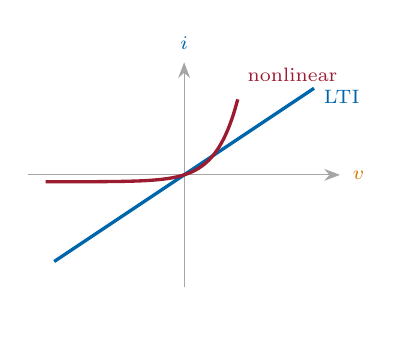
\begin{tikzpicture}[scale=1.1]
        \reviewPlot
      \end{tikzpicture}
    \end{column}
    \begin{column}{0.54\textwidth}
      \begin{itemize}\itemsep8pt
        \item A resistor: a curve in the $v$--$i$ plane
        \item LTI: a line through the origin
        \item Nonlinear: any other curve, e.g.\ $\Icol{i} = g(\Vcol{v})$
        \item So far: LTI circuits only
      \end{itemize}
    \end{column}
  \end{columns}
  \vfill
\end{frame}

%==============================================================
\roadmapframe{1}

%--------------------------------------------------------------
\begin{frame}{Motivation: nonlinear elements}
  \vfill
  \begin{columns}[c,onlytextwidth]
    \begin{column}{0.44\textwidth}
      \centering
      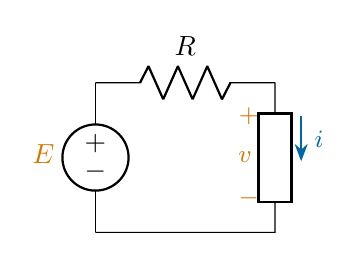
\begin{tikzpicture}[scale=0.95]
        \nlone{$\Vcol{E}$}{$R$}
      \end{tikzpicture}
    \end{column}
    \begin{column}{0.54\textwidth}
      \begin{itemize}\itemsep8pt
        \item Diodes, lamps, transistors: nonlinear
        \item Node and mesh analysis: linear equations
        \item Now: one nonlinear equation, or a few linear pieces
      \end{itemize}
    \end{column}
  \end{columns}
  \vfill
\end{frame}

%--------------------------------------------------------------
\begin{frame}{One nonlinear resistor}
  \begin{columns}[c,onlytextwidth]
    \begin{column}{0.44\textwidth}
      \centering
      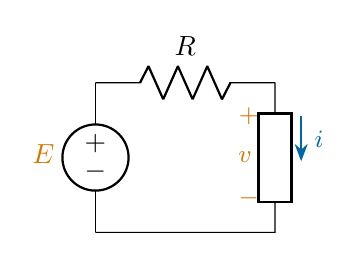
\begin{tikzpicture}[scale=0.95]
        \nlone{$\Vcol{E}$}{$R$}
      \end{tikzpicture}\\[8pt]
      Element: \ $\Icol{i} = g(\Vcol{v})$
    \end{column}
    \begin{column}{0.54\textwidth}
      \textbf{KVL:} \ $E = R\,\Icol{i} + \Vcol{v}$\\[12pt]
      \textbf{Algebraic solution}\\[4pt]
      Solve $E = R\,g(\Vcol{v}) + \Vcol{v}$ for $\Vcol{v_o}$\\[4pt]
      Then $\Icol{i_o} = g(\Vcol{v_o})$\\[12pt]
      Often $g$ is only a measured curve
    \end{column}
  \end{columns}
\end{frame}

%--------------------------------------------------------------
\begin{frame}{The load line}
  \begin{columns}[c,onlytextwidth]
    \begin{column}{0.4\textwidth}
      Two constraints on $(\Vcol{v}, \Icol{i})$:\\[8pt]
      \textcolor{ccur}{circuit:} \ $R\,\Icol{i} + \Vcol{v} = E$\\[4pt]
      \textcolor{metured}{element:} \ $\Icol{i} = g(\Vcol{v})$\\[14pt]
      The solution is on both
    \end{column}
    \begin{column}{0.58\textwidth}
      \centering
      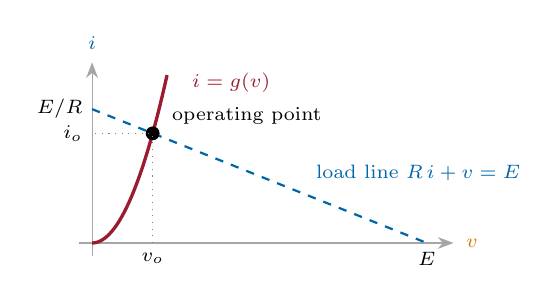
\begin{tikzpicture}[scale=0.85]
        \loadpic
      \end{tikzpicture}
    \end{column}
  \end{columns}
\end{frame}

%--------------------------------------------------------------
\begin{frame}{Example 15.1: the operating point}
  \vfill
  \begin{columns}[c,onlytextwidth]
    \begin{column}{0.44\textwidth}
      \centering
      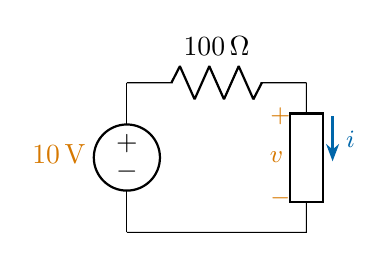
\begin{tikzpicture}[scale=0.95]
        \nlone{$\Vcol{10\V}$}{$100\ohm$}
      \end{tikzpicture}
    \end{column}
    \begin{column}{0.54\textwidth}
      $\Icol{i} = \begin{cases} \frac{3}{100}\,\Vcol{v}^2, & \Vcol{v} \geq 0\\[2pt] 0, & \Vcol{v} < 0 \end{cases}$\\[16pt]
      $(\Vcol{v_o}, \Icol{i_o}) = \ ?$
    \end{column}
  \end{columns}
  \vfill
\end{frame}

%--------------------------------------------------------------
\begin{frame}{Example 15.1: two cases}
  \begin{columns}[c,onlytextwidth]
    \begin{column}{0.5\textwidth}
      \textbf{KVL:} \ $100\,\Icol{i} + \Vcol{v} - 10 = 0$\\[10pt]
      \textbf{$\Vcol{v} < 0$:} \ $\Icol{i} = 0$ \ $\Rightarrow$ \ $\Vcol{v} = 10$\\[2pt]
      \hspace*{1em}contradiction: no solution\\[10pt]
      \onslide<2->{%
      \textbf{$\Vcol{v} \geq 0$:} \ $3\,\Vcol{v}^2 + \Vcol{v} - 10 = 0$\\[2pt]
      \hspace*{1em}$(3\Vcol{v} - 5)(\Vcol{v} + 2) = 0$ \ $\Rightarrow$ \ $\Vcol{v} = \tfrac53\V$\\[12pt]
      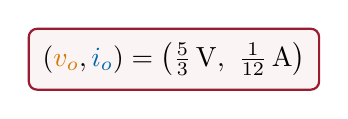
\begin{tikzpicture}
        \node[draw=metured, thick, fill=metured!5, rounded corners=3pt, inner sep=5pt]
          {$(\Vcol{v_o}, \Icol{i_o}) = \big(\tfrac53\V, \ \tfrac{1}{12}\A\big)$};
      \end{tikzpicture}}
    \end{column}
    \begin{column}{0.48\textwidth}
      \centering
      \onslide<2->{%
      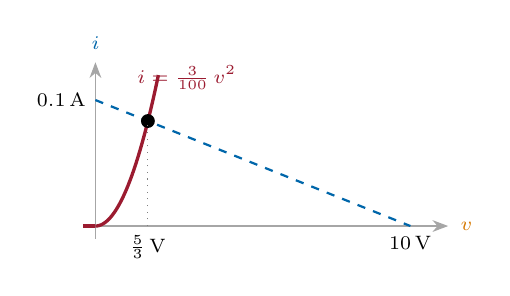
\begin{tikzpicture}[scale=0.8]
        \exOnePlot
      \end{tikzpicture}}
    \end{column}
  \end{columns}
\end{frame}

%--------------------------------------------------------------
\begin{frame}{None, one or many operating points}
  \begin{columns}[t,onlytextwidth]
    \begin{column}{0.48\textwidth}
      \centering
      \textbf{Many}\\[6pt]
      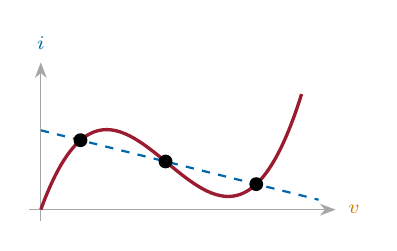
\begin{tikzpicture}[scale=0.72]
        \manypic
      \end{tikzpicture}\\[6pt]
      {\small A bent curve: three intersections}
    \end{column}
    \begin{column}{0.48\textwidth}
      \centering
      \textbf{None}\\[6pt]
      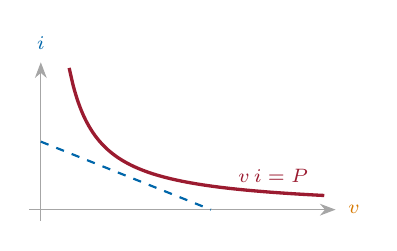
\begin{tikzpicture}[scale=0.72]
        \nonepic
      \end{tikzpicture}\\[6pt]
      {\small No intersection}
    \end{column}
  \end{columns}
  \vfill
  \begin{center}
    A nonlinear circuit need not have exactly one solution
  \end{center}
  \vfill
\end{frame}

%==============================================================
\roadmapframe{3}

%--------------------------------------------------------------
\begin{frame}{A nonlinear resistor in a larger circuit}
  \vfill
  \begin{center}
    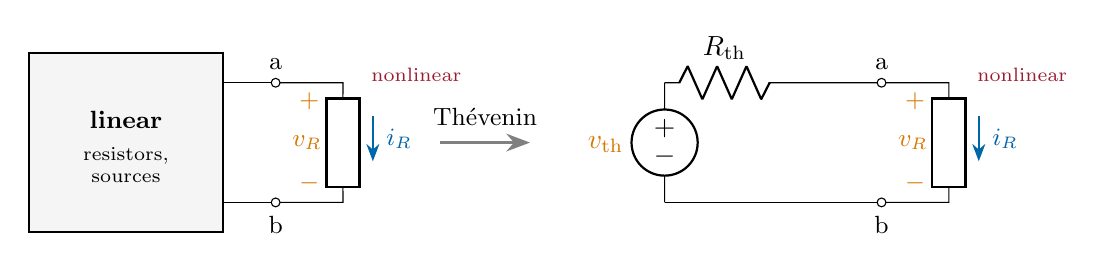
\begin{tikzpicture}[scale=0.95]
      \nlport{0}
      \begin{scope}[visible on=<2->]
        \draw[-{Stealth[length=3mm]}, thick, gray] (5.5,1.2) -- (6.7,1.2);
        \node[font=\small, anchor=south] at (6.1,1.3) {Th\'evenin};
        \begin{scope}[xshift=8.1cm] \nlport{1} \end{scope}
      \end{scope}
    \end{tikzpicture}
  \end{center}
  \vfill
  \begin{center}
    One nonlinear resistor; the rest of the circuit is linear\\[6pt]
    \onslide<2->{Seen from a--b, the rest is a source and a resistor: the case we just solved}
  \end{center}
  \vfill
\end{frame}

%--------------------------------------------------------------
\begin{frame}{Three steps}
  \vfill
  \begin{center}
    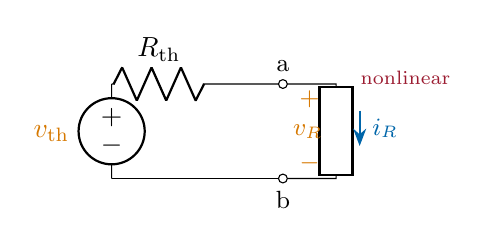
\begin{tikzpicture}[scale=0.75] \nlport{1} \end{tikzpicture}
  \end{center}
  \begin{itemize}\itemsep6pt
    \item \textbf{Step 1:} the Th\'evenin equivalent seen from a--b
    \item \textbf{Step 2:} the load line gives the operating point $(\Vcol{v_R}, \Icol{i_R})$
    \item \textbf{Step 3:} substitution theorem: replace the nonlinear resistor by a source $\Vcol{v_R}$ (or $\Icol{i_R}$)
    \item No other voltage or current changes
    \item Any other voltage or current then follows from a linear circuit
  \end{itemize}
  \vfill
\end{frame}

%--------------------------------------------------------------
\begin{frame}{Example 15.2: find $\Vcol{v}$}
  \vfill
  \begin{columns}[c,onlytextwidth]
    \begin{column}{0.56\textwidth}
      \centering
      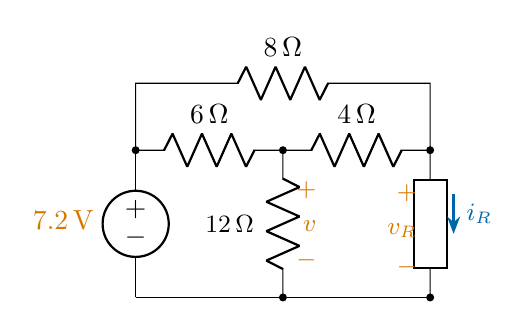
\begin{tikzpicture}[scale=0.85]
        \exTwo{0}
      \end{tikzpicture}
    \end{column}
    \begin{column}{0.42\textwidth}
      $\Icol{i_R} = \begin{cases} \frac14\,\Vcol{v_R}^2, & \Vcol{v_R} \geq 0\\[2pt] 0, & \Vcol{v_R} < 0 \end{cases}$\\[16pt]
      $\Vcol{v} = \ ?$
    \end{column}
  \end{columns}
  \vfill
\end{frame}

%--------------------------------------------------------------
\begin{frame}{Example 15.2: step 1, Th\'evenin}
  \begin{columns}[c,onlytextwidth]
    \begin{column}{0.56\textwidth}
      \centering
      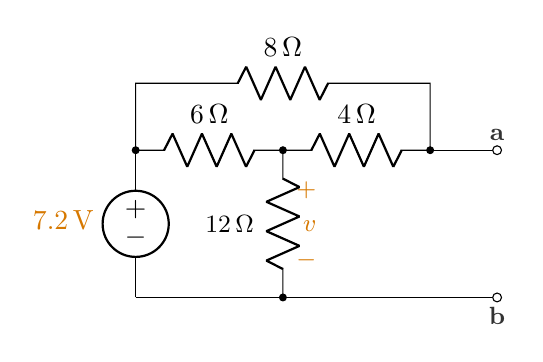
\begin{tikzpicture}[scale=0.85]
        \exTwo{1}
      \end{tikzpicture}
    \end{column}
    \begin{column}{0.42\textwidth}
      \textbf{Kill the source:}\\[4pt]
      $\Rth = 8 \parallel (4 + 6 \parallel 12) = 8 \parallel 8 = 4\ohm$\\[12pt]
      \onslide<2->{%
      \textbf{Open circuit:} two node equations\\[4pt]
      $\vth = \voc = 6\V$\\[12pt]
      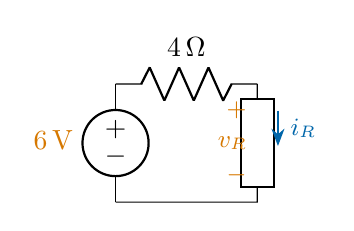
\begin{tikzpicture}[scale=0.75]
        \exTwoTh
      \end{tikzpicture}}
    \end{column}
  \end{columns}
\end{frame}

%--------------------------------------------------------------
\begin{frame}{Example 15.2: step 2, the operating point}
  \begin{columns}[c,onlytextwidth]
    \begin{column}{0.48\textwidth}
      \textbf{KVL:} \ $4\,\Icol{i_R} + \Vcol{v_R} - 6 = 0$\\[8pt]
      Plug $\Icol{i_R} = \tfrac14\,\Vcol{v_R}^2$:\\[4pt]
      $\Vcol{v_R}^2 + \Vcol{v_R} - 6 = 0$\\[4pt]
      $(\Vcol{v_R} + 3)(\Vcol{v_R} - 2) = 0$\\[10pt]
      \onslide<2->{%
      $\Vcol{v_R} \geq 0$: \ $\Vcol{v_R} = 2\V$, \ $\Icol{i_R} = 1\A$}
    \end{column}
    \begin{column}{0.5\textwidth}
      \centering
      \onslide<2->{%
      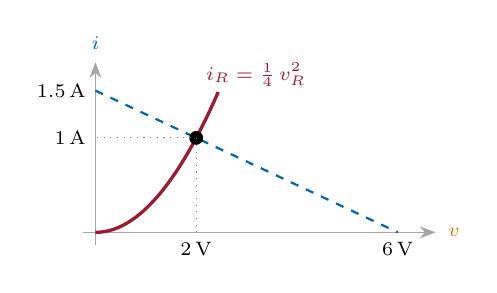
\begin{tikzpicture}[scale=0.8]
        \exTwoPlot
      \end{tikzpicture}}
    \end{column}
  \end{columns}
\end{frame}

%--------------------------------------------------------------
\begin{frame}{Example 15.2: step 3, substitution}
  \begin{columns}[c,onlytextwidth]
    \begin{column}{0.56\textwidth}
      \centering
      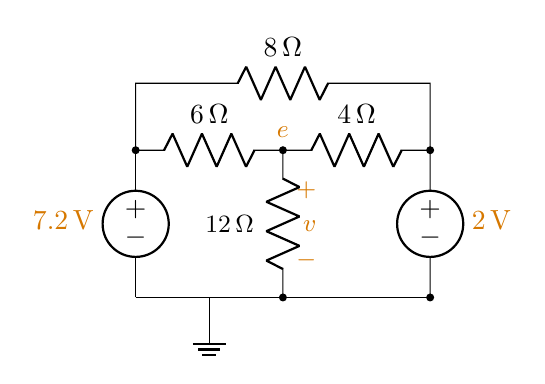
\begin{tikzpicture}[scale=0.85]
        \exTwo{2}
      \end{tikzpicture}
    \end{column}
    \begin{column}{0.42\textwidth}
      Replace it by a $2\V$ source\\[8pt]
      \textbf{Node $\boldsymbol{e}$:}\\[4pt]
      $\dfrac{\e{} - 7.2}{6} + \dfrac{\e{}}{12} + \dfrac{\e{} - 2}{4} = 0$\\[10pt]
      \onslide<2->{%
      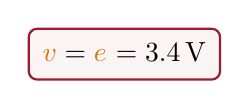
\begin{tikzpicture}
        \node[draw=metured, thick, fill=metured!5, rounded corners=3pt, inner sep=5pt]
          {$\Vcol{v} = \e{} = 3.4\V$};
      \end{tikzpicture}}
    \end{column}
  \end{columns}
\end{frame}

%==============================================================
\roadmapframe{4}

%--------------------------------------------------------------
\begin{frame}{The ideal diode}
  \begin{columns}[c,onlytextwidth]
    \begin{column}{0.3\textwidth}
      \centering
      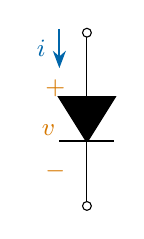
\begin{tikzpicture}[scale=1.0]
        \draw (0,2.2) to[D*] (0,0); \termtb{2.2}
      \end{tikzpicture}
    \end{column}
    \begin{column}{0.34\textwidth}
      \centering
      \begin{tikzpicture}[scale=1.1]
        \ivax{1.6}{1.3}{}
        \draw[crv] (-1.4,0) -- (0,0) -- (0,1.2);
        \node[font=\scriptsize, text=metured, anchor=west] at (0.05,0.9) {ON};
        \node[font=\scriptsize, text=metured, anchor=south] at (-0.8,0.05) {OFF};
      \end{tikzpicture}
    \end{column}
    \begin{column}{0.34\textwidth}
      \textbf{ON:} \ $\Vcol{v} = 0$, \ $\Icol{i} \geq 0$\\[2pt]
      {\small a short circuit}\\[10pt]
      \textbf{OFF:} \ $\Icol{i} = 0$, \ $\Vcol{v} \leq 0$\\[2pt]
      {\small an open circuit}\\[14pt]
      Two straight pieces: \alert{piecewise linear}
    \end{column}
  \end{columns}
\end{frame}

%--------------------------------------------------------------
\begin{frame}{Turning an element around}
  \begin{columns}[c,onlytextwidth]
    \begin{column}{0.5\textwidth}
      \centering
      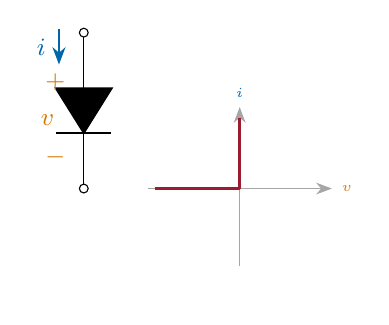
\begin{tikzpicture}[scale=0.9]
        \draw (0,2.2) to[D*] (0,0); \termtb{2.2}
        \begin{scope}[xshift=2.2cm] \pframe{0}{} \pD \end{scope}
      \end{tikzpicture}\\[10pt]
      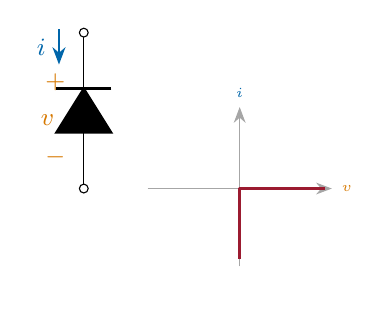
\begin{tikzpicture}[scale=0.9]
        \draw (0,0) to[D*] (0,2.2); \termtb{2.2}
        \begin{scope}[xshift=2.2cm] \pframe{0}{} \pDr \end{scope}
      \end{tikzpicture}
    \end{column}
    \begin{column}{0.48\textwidth}
      Swap the terminals: $\Vcol{v} \to -\Vcol{v}$, \ $\Icol{i} \to -\Icol{i}$\\[12pt]
      The curve is reflected\\ through the origin
    \end{column}
  \end{columns}
\end{frame}

%==============================================================
\begin{frame}{Series and parallel}
  \vfill
  \begin{columns}[t,onlytextwidth]
    \begin{column}{0.48\textwidth}
      \centering
      \textbf{Series:} the same $\Icol{i}$\\[6pt]
      \alert{add the voltages}\\[4pt]
      $\Vcol{v} = \Vcol{v_a} + \Vcol{v_b}$\\[6pt]
      {\small add the curves horizontally}
    \end{column}
    \begin{column}{0.48\textwidth}
      \centering
      \textbf{Parallel:} the same $\Vcol{v}$\\[6pt]
      \alert{add the currents}\\[4pt]
      $\Icol{i} = \Icol{i_a} + \Icol{i_b}$\\[6pt]
      {\small add the curves vertically}
    \end{column}
  \end{columns}
  \vfill
  \begin{center}
    Diodes, LTI resistors and constant sources: the result is piecewise-linear
  \end{center}
  \vfill
\end{frame}

%--------------------------------------------------------------
\begin{frame}{Case I: a resistor and a diode in series}
  \begin{columns}[c,onlytextwidth]
    \begin{column}{0.2\textwidth}
      \centering
      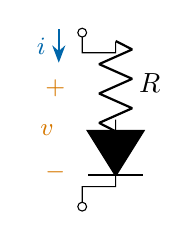
\begin{tikzpicture}[scale=0.85]
        \caseckta
      \end{tikzpicture}
    \end{column}
    \begin{column}{0.78\textwidth}
      \centering
      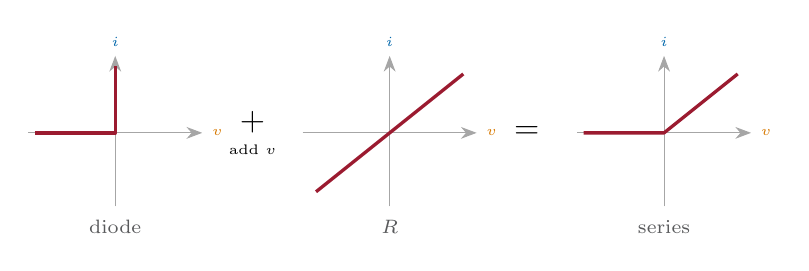
\begin{tikzpicture}[scale=0.85]
        \threeplots{\pD}{\pR{1.1}}{\onslide<2->{\draw[crv] (-1.2,0) -- (0,0) -- (1.1,0.88);}}{\shortstack{$+$\\[1pt]{\tiny add $v$}}}{diode}{$R$}{series}
      \end{tikzpicture}\\[10pt]
      \onslide<2->{$\Icol{i} > 0$: \ $\Vcol{v} = R\,\Icol{i}$; \quad $\Icol{i} = 0$: \ $\Vcol{v} \leq 0$}
    \end{column}
  \end{columns}
\end{frame}

%--------------------------------------------------------------
\begin{frame}{Case II: a resistor and a diode in parallel}
  \begin{columns}[c,onlytextwidth]
    \begin{column}{0.2\textwidth}
      \centering
      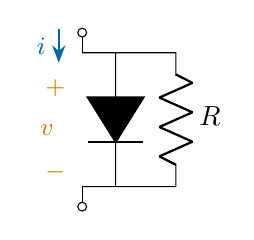
\begin{tikzpicture}[scale=0.85]
        \casecktb
      \end{tikzpicture}
    \end{column}
    \begin{column}{0.78\textwidth}
      \centering
      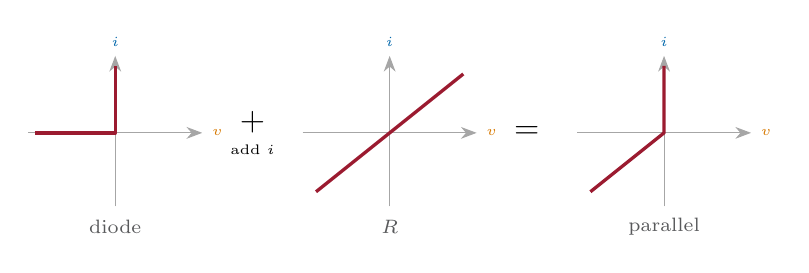
\begin{tikzpicture}[scale=0.85]
        \threeplots{\pD}{\pR{1.1}}{\onslide<2->{\draw[crv] (-1.1,-0.88) -- (0,0) -- (0,1.0);}}{\shortstack{$+$\\[1pt]{\tiny add $i$}}}{diode}{$R$}{parallel}
      \end{tikzpicture}\\[10pt]
      \onslide<2->{$\Vcol{v} < 0$: \ $\Icol{i} = \Vcol{v}/R$; \quad $\Vcol{v} = 0$: \ any $\Icol{i} \geq 0$}
    \end{column}
  \end{columns}
\end{frame}

%--------------------------------------------------------------
\begin{frame}{Reminder: voltage- or current-controlled}
  
  \begin{center}
    \small
    \begin{tabular}{@{}l l l l@{}}
      \textbf{voltage-controlled} & $\Icol{i} = g(\Vcol{v})$ & vertical lines: once & $\to$ KCL, node analysis\\[2pt]
      \textbf{current-controlled} & $\Vcol{v} = r(\Icol{i})$ & horizontal lines: once & $\to$ KVL, mesh analysis\\[2pt]
      \textbf{neither} & & & $\to$ assume ON or OFF
    \end{tabular}
  \end{center}
  \vspace{-4pt}
  \begin{center}
  \begin{tabular}{@{}>{\centering}p{3.3cm} >{\centering}p{3.3cm} >{\centering\arraybackslash}p{3.3cm}@{}}
    \shortstack{\scell{\cR}{resistor}{both}} &
    \shortstack{\scell{\cI}{current source}{voltage-controlled}} &
    \shortstack{\scell{\cE}{voltage source}{current-controlled}}\\[0pt]
    \shortstack{\scell{\pD}{ideal diode}{neither}} &
    \shortstack{\scell{\caseresa}{Case I: $R$ in series}{voltage-controlled}} &
    \shortstack{\scell{\caseresb}{Case II: $R$ in parallel}{current-controlled}}
  \end{tabular}
  \end{center}
\end{frame}

%--------------------------------------------------------------
\begin{frame}{Example 15.3: a diode, a resistor and a source}
  \vfill
  \begin{columns}[c,onlytextwidth]
    \begin{column}{0.4\textwidth}
      \centering
      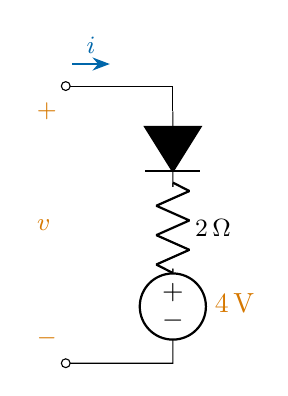
\begin{tikzpicture}[scale=0.8]
        \exS{0}
      \end{tikzpicture}
    \end{column}
    \begin{column}{0.58\textwidth}
      $\Icol{i}$ as a function of $\Vcol{v}$ \ $= \ ?$\\[14pt]
      \textbf{Method:} assume a state for the diode\\[4pt]
      Solve the linear circuit\\[4pt]
      Keep the result where the assumption holds
    \end{column}
  \end{columns}
  \vfill
\end{frame}

%--------------------------------------------------------------
\begin{frame}{Example 15.3: assume the diode ON}
  \begin{columns}[c,onlytextwidth]
    \begin{column}{0.4\textwidth}
      \centering
      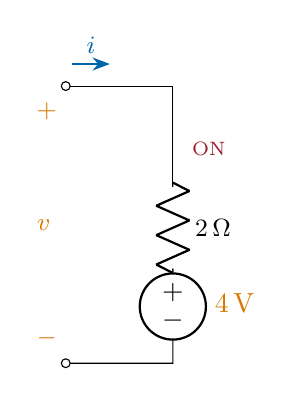
\begin{tikzpicture}[scale=0.8]
        \exS{1}
      \end{tikzpicture}
    \end{column}
    \begin{column}{0.58\textwidth}
      ON: a short; \ condition $\Icol{i} \geq 0$\\[10pt]
      KVL: \ $\Vcol{v} = 2\,\Icol{i} + 4$\\[10pt]
      \onslide<2->{%
      $\Icol{i} = \dfrac{\Vcol{v} - 4}{2} \geq 0$ \ $\Leftrightarrow$ \ \alert{$\Vcol{v} \geq 4\V$}}
    \end{column}
  \end{columns}
\end{frame}

%--------------------------------------------------------------
\begin{frame}{Example 15.3: assume the diode OFF}
  \begin{columns}[c,onlytextwidth]
    \begin{column}{0.4\textwidth}
      \centering
      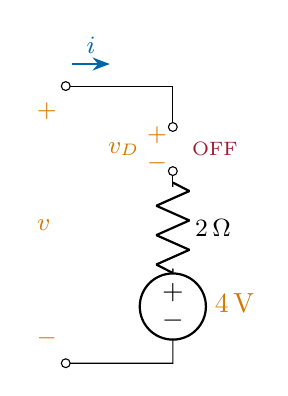
\begin{tikzpicture}[scale=0.8]
        \exS{2}
      \end{tikzpicture}
    \end{column}
    \begin{column}{0.58\textwidth}
      OFF: an open; \ condition $\Vcol{v_D} < 0$\\[10pt]
      $\Icol{i} = 0$: \ no voltage on $2\ohm$\\[10pt]
      \onslide<2->{%
      KVL: \ $\Vcol{v_D} = \Vcol{v} - 4$\\[8pt]
      $\Vcol{v_D} < 0$ \ $\Leftrightarrow$ \ \alert{$\Vcol{v} < 4\V$}}
    \end{column}
  \end{columns}
\end{frame}

%--------------------------------------------------------------
\begin{frame}{Example 15.3: the result}
  \begin{columns}[c,onlytextwidth]
    \begin{column}{0.46\textwidth}
      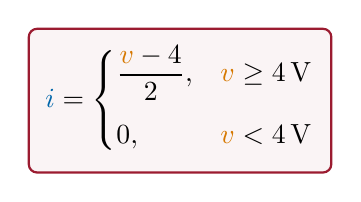
\begin{tikzpicture}
        \node[draw=metured, thick, fill=metured!5, rounded corners=3pt, inner sep=6pt]
          {$\Icol{i} = \begin{cases} \dfrac{\Vcol{v} - 4}{2}, & \Vcol{v} \geq 4\V\\[8pt] 0, & \Vcol{v} < 4\V \end{cases}$};
      \end{tikzpicture}\\[12pt]
      Breakpoint: \ $\Icol{i_D} = 0$ and $\Vcol{v_D} = 0$
    \end{column}
    \begin{column}{0.52\textwidth}
      \centering
      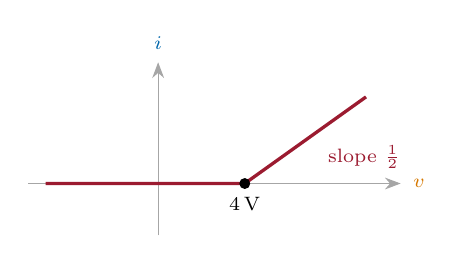
\begin{tikzpicture}[scale=1.1]
        \exSPlot
      \end{tikzpicture}
    \end{column}
  \end{columns}
\end{frame}

%--------------------------------------------------------------
\begin{frame}{Example 15.3: graphically}
  \vfill
  \begin{center}
    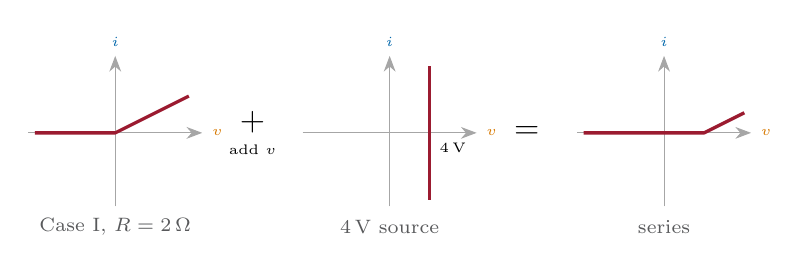
\begin{tikzpicture}[scale=0.85]
      \threeplots{\draw[crv] (-1.2,0) -- (0,0) -- (1.1,0.55);}{\draw[crv] (0.6,-1.0) -- (0.6,1.0); \node[font=\tiny, below right] at (0.6,0) {$4\V$};}{\onslide<2->{\draw[crv] (-1.2,0) -- (0.6,0) -- (1.2,0.3);}}{\shortstack{$+$\\[1pt]{\tiny add $v$}}}{Case I, $R = 2\ohm$}{$4\V$ source}{series}
    \end{tikzpicture}
  \end{center}
  \vfill
  \begin{center}
    \onslide<2->{A source in series shifts the curve right by $4\V$ \ \yes}
  \end{center}
  \vfill
\end{frame}

%--------------------------------------------------------------
\begin{frame}{Case III: combinations}
  \begin{columns}[c,onlytextwidth]
    \begin{column}{0.2\textwidth}
      \centering
      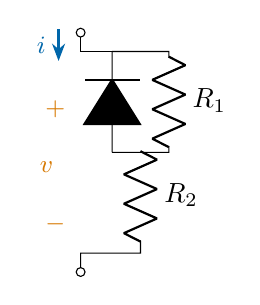
\begin{tikzpicture}[scale=0.8]
        \casecktc
      \end{tikzpicture}
    \end{column}
    \begin{column}{0.78\textwidth}
      \centering
      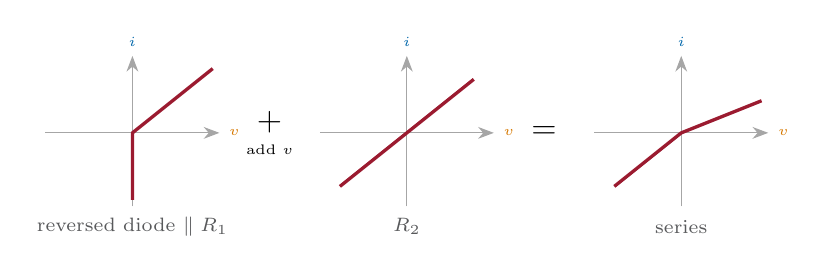
\begin{tikzpicture}[scale=0.85]
        \threeplots{\draw[crv] (0,-1.0) -- (0,0) -- (1.2,0.96);}{\pR{1.0}}{\onslide<2->{\draw[crv] (-1.0,-0.8) -- (0,0) -- (1.2,0.48);}}{\shortstack{$+$\\[1pt]{\tiny add $v$}}}{reversed diode $\parallel R_1$}{$R_2$}{series}
      \end{tikzpicture}\\[10pt]
      {\small For simplicity, $R_1 = R_2 = R$.}\\[6pt]
      \onslide<2->{$\Icol{i} > 0$: diode OFF, \ slope $\dfrac{1}{2R}$; \quad $\Icol{i} < 0$: diode ON, \ slope $\dfrac{1}{R}$}
    \end{column}
  \end{columns}
\end{frame}

%--------------------------------------------------------------
\begin{frame}{Case IV: combinations}
  \begin{columns}[c,onlytextwidth]
    \begin{column}{0.2\textwidth}
      \centering
      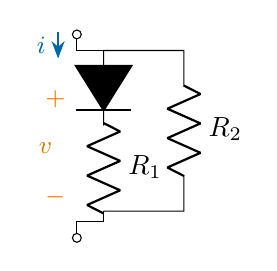
\begin{tikzpicture}[scale=0.68]
        \casecktd
      \end{tikzpicture}
    \end{column}
    \begin{column}{0.78\textwidth}
      \centering
      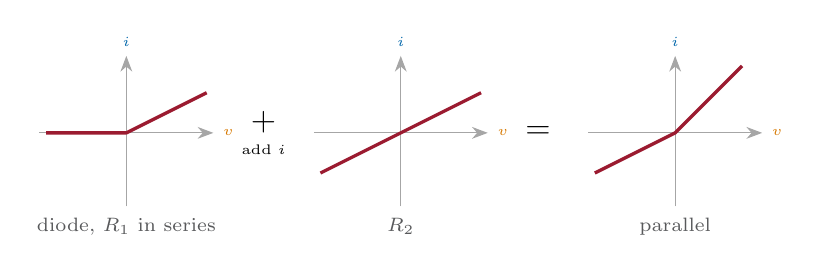
\begin{tikzpicture}[scale=0.85]
        \threeplots{\draw[crv] (-1.2,0) -- (0,0) -- (1.2,0.6);}{\draw[crv] (-1.2,-0.6) -- (1.2,0.6);}{\onslide<2->{\draw[crv] (-1.2,-0.6) -- (0,0) -- (1.0,1.0);}}{\shortstack{$+$\\[1pt]{\tiny add $i$}}}{diode, $R_1$ in series}{$R_2$}{parallel}
      \end{tikzpicture}\\[10pt]
      {\small For simplicity, $R_1 = R_2 = R$.}\\[6pt]
      \onslide<2->{$\Vcol{v} > 0$: slope $\dfrac{2}{R}$; \quad $\Vcol{v} < 0$: slope $\dfrac{1}{R}$}
    \end{column}
  \end{columns}
\end{frame}

%--------------------------------------------------------------
\begin{frame}{Case V: a diode and a voltage source in series}
  \begin{columns}[c,onlytextwidth]
    \begin{column}{0.2\textwidth}
      \centering
      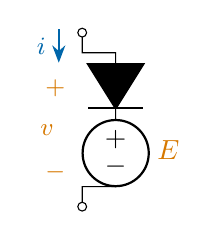
\begin{tikzpicture}[scale=0.85]
        \caseckte
      \end{tikzpicture}
    \end{column}
    \begin{column}{0.78\textwidth}
      \centering
      \begin{tikzpicture}[scale=0.85]
        \threeplots{\pD}{\draw[crv] (0.6,-1.0) -- (0.6,1.0); \node[font=\tiny, below right] at (0.6,0) {$E$};}{\onslide<2->{\draw[crv] (-1.2,0) -- (0.6,0) -- (0.6,1.0); \node[font=\tiny, below] at (0.6,0) {$E$};}}{\shortstack{$+$\\[1pt]{\tiny add $v$}}}{diode}{source}{series}
      \end{tikzpicture}\\[10pt]
      \onslide<2->{The diode curve shifted right by $E$}
    \end{column}
  \end{columns}
\end{frame}

%--------------------------------------------------------------
\begin{frame}{Case VI: a diode and a current source in parallel}
  \begin{columns}[c,onlytextwidth]
    \begin{column}{0.2\textwidth}
      \centering
      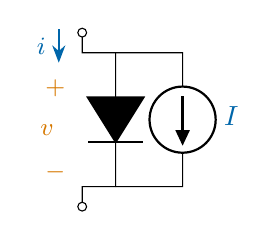
\begin{tikzpicture}[scale=0.85]
        \casecktf
      \end{tikzpicture}
    \end{column}
    \begin{column}{0.78\textwidth}
      \centering
      \begin{tikzpicture}[scale=0.85]
        \threeplots{\pD}{\draw[crv] (-1.2,0.5) -- (1.2,0.5); \node[font=\tiny, above right] at (0,0.5) {$I$};}{\onslide<2->{\draw[crv] (-1.2,0.5) -- (0,0.5) -- (0,1.05); \node[font=\tiny, left] at (0,0.5) {$I$};}}{\shortstack{$+$\\[1pt]{\tiny add $i$}}}{diode}{source}{parallel}
      \end{tikzpicture}\\[10pt]
      \onslide<2->{The diode curve shifted up by $I$}
    \end{column}
  \end{columns}
\end{frame}

%--------------------------------------------------------------
\begin{frame}{Case VII: sources and a diode}
  \begin{columns}[c,onlytextwidth]
    \begin{column}{0.2\textwidth}
      \centering
      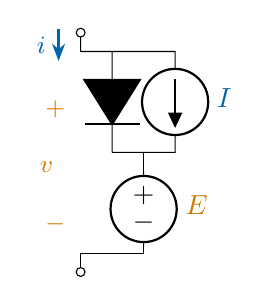
\begin{tikzpicture}[scale=0.8]
        \casecktg
      \end{tikzpicture}
    \end{column}
    \begin{column}{0.78\textwidth}
      \centering
      \begin{tikzpicture}[scale=0.85]
        \threeplots{\draw[crv] (-1.2,0.5) -- (0,0.5) -- (0,1.05);}{\draw[crv] (0.6,-1.0) -- (0.6,1.0); \node[font=\tiny, below right] at (0.6,0) {$E$};}{\onslide<2->{\draw[crv] (-1.2,0.5) -- (0.6,0.5) -- (0.6,1.05); \node[font=\tiny, below] at (0.6,0) {$E$};}}{\shortstack{$+$\\[1pt]{\tiny add $v$}}}{Case VI}{source}{series}
      \end{tikzpicture}\\[10pt]
      \onslide<2->{The source has $+$ at the top: \ shifted right by $E$}
    \end{column}
  \end{columns}
\end{frame}

%--------------------------------------------------------------
\begin{frame}{The ideal Zener diode}
  \begin{columns}[c,onlytextwidth]
    \begin{column}{0.14\textwidth}
      \centering
      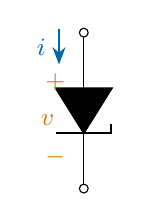
\begin{tikzpicture}[scale=0.9]
        \draw (0,2.2) to[zD*] (0,0); \termtb{2.2}
      \end{tikzpicture}
    \end{column}
    \begin{column}{0.3\textwidth}
      \centering
      \begin{tikzpicture}[scale=0.95]
        \zenerPlot
      \end{tikzpicture}
    \end{column}
    \begin{column}{0.24\textwidth}
      \centering
      \onslide<2->{%
      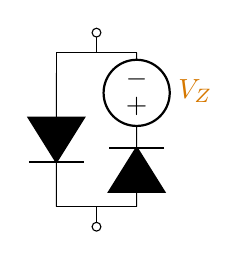
\begin{tikzpicture}[scale=0.85]
        \zenerEq
      \end{tikzpicture}}
    \end{column}
    \begin{column}{0.3\textwidth}
      Forward: like a diode\\[6pt]
      Reverse: blocks until $\Vcol{v} = -V_Z$\\[12pt]
      \onslide<2->{Two diodes and a battery $V_Z$}
    \end{column}
  \end{columns}
\end{frame}

%==============================================================
\roadmapframe{6}

%--------------------------------------------------------------
\begin{frame}{Example 15.4: two diodes}
  \vfill
  \begin{columns}[c,onlytextwidth]
    \begin{column}{0.5\textwidth}
      \centering
      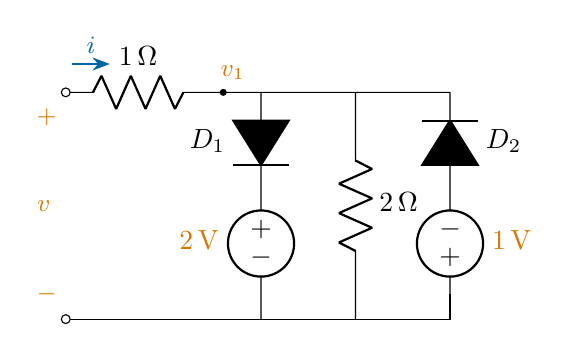
\begin{tikzpicture}[scale=0.8]
        \exH
      \end{tikzpicture}
    \end{column}
    \begin{column}{0.48\textwidth}
      $\Icol{i}$ as a function of $\Vcol{v}$ \ $= \ ?$\\[14pt]
      Two diodes: four combinations\\[4pt]
      One linear circuit for each\\[4pt]
      Keep each result where it is valid
    \end{column}
  \end{columns}
  \vfill
\end{frame}

%--------------------------------------------------------------
\begin{frame}{Example 15.4: both diodes OFF}
  \begin{columns}[c,onlytextwidth]
    \begin{column}{0.5\textwidth}
      \centering
      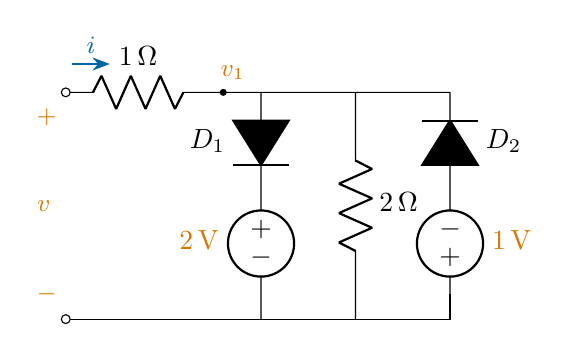
\begin{tikzpicture}[scale=0.8]
        \exH
      \end{tikzpicture}
    \end{column}
    \begin{column}{0.48\textwidth}
      $1\ohm$ and $2\ohm$ in series:\\[4pt]
      $\Vcol{v_1} = 2\,\Icol{i}$, \quad $\Vcol{v} = 3\,\Icol{i}$\\[12pt]
      \onslide<2->{%
      $D_1$ OFF: \ $\Vcol{v_{D_1}} = \Vcol{v_1} - 2 < 0$\\[4pt]
      $D_2$ OFF: \ $\Vcol{v_{D_2}} = -1 - \Vcol{v_1} < 0$\\[8pt]
      $-1 < \Vcol{v_1} < 2$ \ $\Leftrightarrow$ \ \alert{$-1.5 < \Vcol{v} < 3$}}
    \end{column}
  \end{columns}
\end{frame}

%--------------------------------------------------------------
\begin{frame}{Example 15.4: $D_1$ ON, $D_2$ OFF}
  \begin{columns}[c,onlytextwidth]
    \begin{column}{0.5\textwidth}
      \centering
      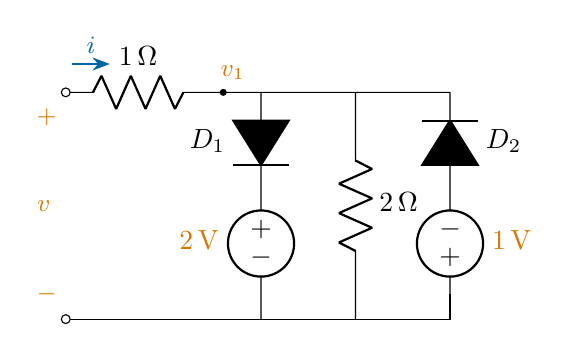
\begin{tikzpicture}[scale=0.8]
        \exH
      \end{tikzpicture}
    \end{column}
    \begin{column}{0.48\textwidth}
      $D_1$ a short: \ $\Vcol{v_1} = 2$\\[4pt]
      $\Vcol{v} = \Icol{i} + 2$\\[12pt]
      \onslide<2->{%
      $2\ohm$: $1\A$; \ $D_1$: $\Icol{i_{D_1}} = \Icol{i} - 1$\\[4pt]
      $\Icol{i_{D_1}} \geq 0$ \ $\Leftrightarrow$ \ \alert{$\Vcol{v} \geq 3$}\\[8pt]
      $D_2$: \ $\Vcol{v_{D_2}} = -1 - 2 < 0$ \ \yes}
    \end{column}
  \end{columns}
\end{frame}

%--------------------------------------------------------------
\begin{frame}{Example 15.4: $D_2$ ON, $D_1$ OFF}
  \begin{columns}[c,onlytextwidth]
    \begin{column}{0.5\textwidth}
      \centering
      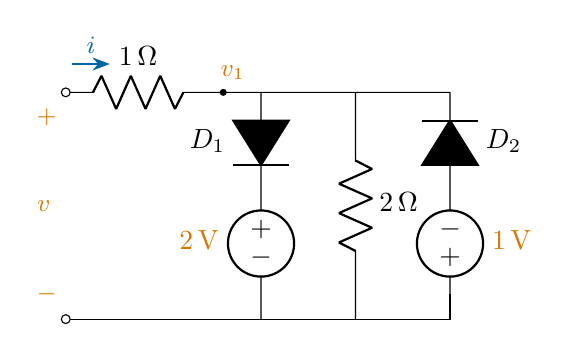
\begin{tikzpicture}[scale=0.8]
        \exH
      \end{tikzpicture}
    \end{column}
    \begin{column}{0.48\textwidth}
      $D_2$ a short: \ $\Vcol{v_1} = -1$\\[4pt]
      $\Vcol{v} = \Icol{i} - 1$\\[12pt]
      \onslide<2->{%
      $2\ohm$: $-0.5\A$; \ $D_2$: $\Icol{i_{D_2}} = -0.5 - \Icol{i}$\\[4pt]
      $\Icol{i_{D_2}} \geq 0$ \ $\Leftrightarrow$ \ \alert{$\Vcol{v} \leq -1.5$}\\[8pt]
      $D_1$: \ $\Vcol{v_{D_1}} = -1 - 2 < 0$ \ \yes}
    \end{column}
  \end{columns}
\end{frame}

%--------------------------------------------------------------
\begin{frame}{Example 15.4: the result}
  \begin{columns}[c,onlytextwidth]
    \begin{column}{0.5\textwidth}
      Both ON: \ $\Vcol{v_1} = 2$ and $-1$ \ (impossible)\\[12pt]
      \begin{tikzpicture}
        \node[draw=metured, thick, fill=metured!5, rounded corners=3pt, inner sep=6pt]
          {$\Icol{i} = \begin{cases} \Vcol{v} - 2, & \Vcol{v} \geq 3\\[4pt] \Vcol{v}/3, & -1.5 \leq \Vcol{v} \leq 3\\[4pt] \Vcol{v} + 1, & \Vcol{v} \leq -1.5 \end{cases}$};
      \end{tikzpicture}\\[10pt]
      Two diodes: two breakpoints
    \end{column}
    \begin{column}{0.48\textwidth}
      \centering
      \begin{tikzpicture}[scale=1.0]
        \exHPlot
      \end{tikzpicture}
    \end{column}
  \end{columns}
\end{frame}

%--------------------------------------------------------------
\begin{frame}{Example 15.4: graphically}
  \vfill
  \begin{center}
    \begin{tikzpicture}[scale=0.7]
      \begin{scope}\pframe{0}{$D_1$, $2\V$} \draw[crv] (-1.2,0) -- (0.8,0) -- (0.8,1.05); \end{scope}
      \node[font=\large] at (1.9,0) {\shortstack{$+$\\[1pt]{\tiny add $i$}}};
      \begin{scope}[xshift=3.8cm]\pframe{0}{$2\ohm$} \draw[crv] (-1.1,-0.55) -- (1.1,0.55); \end{scope}
      \node[font=\large] at (5.7,0) {\shortstack{$+$\\[1pt]{\tiny add $i$}}};
      \begin{scope}[xshift=7.6cm]\pframe{0}{$D_2$, $1\V$} \draw[crv] (-0.4,-1.0) -- (-0.4,0) -- (1.2,0); \end{scope}
      \node[font=\large] at (9.5,0) {$=$};
      \begin{scope}[xshift=11.4cm]\pframe{0}{parallel part} \draw[crv] (-0.4,-1.0) -- (-0.4,-0.2) -- (0.8,0.4) -- (0.8,1.05); \end{scope}
    \end{tikzpicture}\\[16pt]
    \onslide<2->{%
    \begin{tikzpicture}[scale=0.7]
      \threeplots{\draw[crv] (-0.4,-1.0) -- (-0.4,-0.2) -- (0.8,0.4) -- (0.8,1.05);}{\pR{1.0}}{\draw[crv] (-1.2,-0.85) -- (-0.75,-0.25) -- (0.75,0.25) -- (1.2,0.85);}{\shortstack{$+$\\[1pt]{\tiny add $v$}}}{parallel part}{$1\ohm$}{the one-port}
    \end{tikzpicture}}
  \end{center}
  \vfill
\end{frame}

%==============================================================
\roadmapframe{7}

%--------------------------------------------------------------
\begin{frame}{Example 15.5: a circuit from a characteristic}
  \vfill
  \begin{columns}[c,onlytextwidth]
    \begin{column}{0.5\textwidth}
      \centering
      \begin{tikzpicture}[scale=1.05]
        \synPlot
      \end{tikzpicture}
    \end{column}
    \begin{column}{0.48\textwidth}
      A circuit with this $i$--$v$ characteristic $= \ ?$\\[14pt]
      \onslide<2->{%
      One breakpoint: \ one diode\\[4pt]
      Below $2\V$: \ a line through the origin}
    \end{column}
  \end{columns}
  \vfill
\end{frame}

%--------------------------------------------------------------
\begin{frame}{Example 15.5: split the characteristic}
  \vfill
  \begin{center}
    \begin{tikzpicture}[scale=0.85]
      \threeplots{\draw[crv] (-1.2,-0.3) -- (1.2,0.3);}{\draw[crv] (-1.2,0) -- (0.4,0) -- (1.2,0.4); \node[font=\tiny, below] at (0.4,0) {$2\V$};}{\draw[crv] (-1.2,-0.3) -- (0.4,0.1) -- (1.2,0.7);}{\shortstack{$+$\\[1pt]{\tiny add $i$}}}{$4\ohm$}{slope $\tfrac12$ after $2\V$}{target}
    \end{tikzpicture}
  \end{center}
  \vfill
  \begin{itemize}\itemsep8pt
    \item Slope $\tfrac14\Sie$ everywhere: \ a $4\ohm$ resistor
    \item Extra slope $\tfrac34 - \tfrac14 = \tfrac12\Sie$ after $2\V$: \ Case I with $2\ohm$, shifted by $2\V$
    \item Currents add: \ the two in parallel
  \end{itemize}
  \vfill
\end{frame}

%--------------------------------------------------------------
\begin{frame}{Example 15.5: the circuit}
  \begin{columns}[c,onlytextwidth]
    \begin{column}{0.4\textwidth}
      \centering
      \begin{tikzpicture}[scale=0.75]
        \synCkt
      \end{tikzpicture}
    \end{column}
    \begin{column}{0.58\textwidth}
      Check at $\Vcol{v} = 4\V$:\\[4pt]
      $4\ohm$: $1\A$; \ branch: $\dfrac{4 - 2}{2} = 1\A$\\[4pt]
      $\Icol{i} = 2\A$ \ \yes\\[14pt]
      The order inside the branch does not matter:\\[2pt]
      the circuit is \alert{not unique}
    \end{column}
  \end{columns}
\end{frame}

%--------------------------------------------------------------
\begin{frame}{Example 15.6: a circuit from a characteristic}
  \begin{columns}[c,onlytextwidth]
    \begin{column}{0.46\textwidth}
      \centering
      \begin{tikzpicture}[scale=1.0]
        \exFourPlot
      \end{tikzpicture}
    \end{column}
    \begin{column}{0.52\textwidth}
      A circuit with this $i$--$v$ characteristic $= \ ?$\\[12pt]
      \onslide<2->{%
      Two breakpoints: \ at least two diodes\\[8pt]
      Split into pieces we know}
    \end{column}
  \end{columns}
\end{frame}

%--------------------------------------------------------------
\begin{frame}{Example 15.6: split the characteristic}
  \vfill
  \begin{center}
    \begin{tikzpicture}[scale=0.78]
      \begin{scope}\pframe{0}{target} \draw[crv] (-1.2,-0.8) -- (0,0) -- (0,0.5) -- (1.2,1.0); \end{scope}
      \node[font=\large] at (2.05,0) {$=$};
      \begin{scope}[xshift=4.1cm]\pframe{0}{A: diode $\parallel 1\ohm$} \draw[crv] (-1.2,-0.8) -- (0,0) -- (0,1.0); \end{scope}
      \node[font=\large] at (6.15,0) {\shortstack{$+$\\[1pt]{\tiny add $v$}}};
      \begin{scope}[xshift=8.2cm]\pframe{0}{B} \draw[crv] (0,-1.0) -- (0,0.5) -- (1.2,1.0); \end{scope}
    \end{tikzpicture}\\[18pt]
    \onslide<2->{%
    \begin{tikzpicture}[scale=0.78]
      \begin{scope}\pframe{0}{B} \draw[crv] (0,-1.0) -- (0,0.5) -- (1.2,1.0); \end{scope}
      \node[font=\large] at (2.05,0) {$=$};
      \begin{scope}[xshift=4.1cm]\pframe{0}{reversed diode $\parallel 2\ohm$} \draw[crv] (0,-1.0) -- (0,0) -- (1.2,0.5); \end{scope}
      \node[font=\large] at (6.15,0) {\shortstack{$+$\\[1pt]{\tiny add $i$}}};
      \begin{scope}[xshift=8.2cm]\pframe{0}{source $1\A$} \draw[crv] (-1.2,0.5) -- (1.2,0.5); \end{scope}
    \end{tikzpicture}}
  \end{center}
  \vfill
\end{frame}

%--------------------------------------------------------------
\begin{frame}{Example 15.6: the circuit}
  \begin{columns}[c,onlytextwidth]
    \begin{column}{0.4\textwidth}
      \centering
      \begin{tikzpicture}[scale=0.78]
        \exFourCkt
      \end{tikzpicture}
    \end{column}
    \begin{column}{0.58\textwidth}
      Top: A, \ the diode $\parallel 1\ohm$\\[6pt]
      Bottom: B, \ reversed diode $\parallel 2\ohm \parallel 1\A$\\[6pt]
      A and B in series\\[6pt]
      Check at $\Vcol{v} = 2\V$: \ $\Icol{i} = 1 + \tfrac22 = 2\A$ \ \yes\\[12pt]
      Another circuit may have the same characteristic:\\[2pt]
      the circuit is \alert{not unique}
    \end{column}
  \end{columns}
\end{frame}

%--------------------------------------------------------------
\begin{frame}{Example 15.7: a numerical characteristic}
  \begin{columns}[c,onlytextwidth]
    \begin{column}{0.46\textwidth}
      \centering
      \begin{tikzpicture}[scale=1.0]
        \exFivePlot
      \end{tikzpicture}
    \end{column}
    \begin{column}{0.52\textwidth}
      Slopes $2\Sie$, $1\Sie$, $2\Sie$\\[8pt]
      A circuit $= \ ?$\\[12pt]
      \onslide<2->{%
      \textbf{Split} (parallel, add currents):\\[4pt]
      a $1\ohm$ resistor\\[2pt]
      $+$ \ a $1\Sie$ branch for $\Vcol{v} > 2\V$\\[2pt]
      $+$ \ a $1\Sie$ branch for $\Vcol{v} < -2\V$}
    \end{column}
  \end{columns}
\end{frame}

%--------------------------------------------------------------
\begin{frame}{Example 15.7: the circuit}
  \begin{columns}[c,onlytextwidth]
    \begin{column}{0.56\textwidth}
      \centering
      \begin{tikzpicture}[scale=0.72]
        \exFiveCkt
      \end{tikzpicture}
    \end{column}
    \begin{column}{0.42\textwidth}
      Branch 2: \ $\Vcol{v} - 2$ \ for $\Vcol{v} > 2\V$\\[8pt]
      Branch 3: turned around\\[4pt]
      \hspace*{1em}$\Vcol{v} + 2$ \ for $\Vcol{v} < -2\V$\\[12pt]
      \onslide<2->{%
      Check at $\Vcol{v} = 3\V$:\\[2pt]
      $3 + 1 + 0 = 4\A$ \ \yes}
    \end{column}
  \end{columns}
\end{frame}

%==============================================================
\roadmapframe{8}

%--------------------------------------------------------------
\begin{frame}{Example 15.8: a linear time-varying circuit}
  \begin{columns}[c,onlytextwidth]
    \begin{column}{0.5\textwidth}
      \centering
      \begin{tikzpicture}[scale=0.85]
        \exSix
      \end{tikzpicture}\\[8pt]
      {\small $R_1(t)$, $R_2(t)$: linear, time-varying}
    \end{column}
    \begin{column}{0.48\textwidth}
      \textbf{KCL:} \ $\dfrac{\Vcol{v} - \Vcol{v_s}}{R_1} - \Icol{i_s} + \dfrac{\Vcol{v}}{R_2} = 0$\\[12pt]
      \onslide<2->{%
      $\Vcol{v} = \underbrace{\dfrac{R_2}{R_1 + R_2}}_{k_1(t)}\Vcol{v_s} + \underbrace{\dfrac{R_1R_2}{R_1 + R_2}}_{k_2(t)}\Icol{i_s}$\\[12pt]}
      \onslide<2->{%
      $\Vcol{v} = \mathbf{k}(t)\,\mathbf{u}$: \ superposition still holds}
    \end{column}
  \end{columns}
\end{frame}

%--------------------------------------------------------------
\begin{frame}{Summary}
  \vfill
  \begin{center}
  \renewcommand{\arraystretch}{1.55}
  \begin{tabular}{@{}>{\raggedright}p{4.2cm} >{\raggedright\arraybackslash}p{8.0cm}@{}}
    \toprule
    \textbf{In the circuit} & \textbf{What to do}\\
    \midrule
    one nonlinear resistor & load line $R\,\Icol{i} + \Vcol{v} = E$ meets $\Icol{i} = g(\Vcol{v})$\\
    a linear rest & Th\'evenin, operating point, substitution\\
    ideal diodes & assume ON / OFF, solve, check\\
    series, parallel & add voltages, add currents\\
    a given characteristic & split it into known pieces\\
    linear time-varying & $\Vcol{v} = \mathbf{k}(t)\,\mathbf{u}$: superposition holds\\
    \bottomrule
  \end{tabular}
  \end{center}
  \vfill
\end{frame}

\end{document}
